
\section{Méthodologie et mise en œuvre}


Dans cette partie, on décrit l'ensemble des travaux réalisés au cours de ce stage, 
organisés selon une progression logique allant de la reconstruction de 
la scène 3D jusqu'à l'approche continue d'apprentissage par renforcement pour la navigation visuelle.

Nous commençons par la reconstruction de la scène \textit{room} à l'aide 
du 3D Gaussian Splatting (section~\ref{sec:reconstruction}), qui constitue 
le base visuelle de l'ensemble du pipeline. Nous reproduisons ensuite le 
pipeline de navigation visuelle issu des travaux de Zhu et al. \cite{ref10} sur les scènes AI2-THOR, afin de valider notre approche et notre environnement d'apprentissage (section~\ref{sec:aithor}). Nous adaptons ensuite ce pipeline à notre scène 3DGS en construisant un graphe de navigation discret et en réentraînant l'agent A3C sur la scène 
\textit{room} (section~\ref{sec:graphe_room}). Enfin, nous présentons l'extension vers une approche de navigation 
continue (section~\ref{sec:approche_continue}), dans laquelle l'espace 
d'actions discret est remplacé par un espace continu, et où nous 
comparons les performances des algorithmes A3C et PPO en utilisant 
des caractéristiques visuelles extraites par un réseau ResNet-18 
pré-entraîné comme représentation de l'état de l'agent.


\subsection{Reconstruction de la scène avec 3DGS}
\label{sec:reconstruction}



Dans cette section, on utilise les 311 images et les poses COLMAP de la 
séquence \textit{room} de Mip-NeRF 360 pour entraîner un modèle Splatfacto 
(via Nerfstudio) sur le cluster HPC Toubkal/Kaggle.

Les images sont d'abord sous-échantillonnées d'un facteur 4 
(\texttt{images\_4/}) pour garantir un  coût computationnel réduit tout en conservant qualité d'apprentissage.

Le pipeline de reconstruction suit les étapes suivantes :

\begin{enumerate}[noitemsep, topsep=4pt]
    \item \textbf{Données d'entrée} : les 311 images RGB et les poses 
    de caméra associées (position + orientation), issues du dataset 
    Mip-NeRF 360.
    \item \textbf{Découpage train/test} : les images sont séparées en 
    un ensemble d'entraînement et un ensemble de test, suivant le 
    protocole standard de Nerfstudio.
    \item \textbf{Entraînement Splatfacto} : le modèle 3DGS est entraîné 
    sur les images d'entraînement via le modèle Splatfacto de Nerfstudio, 
    sur le cluster HPC Toubkal sur 30 000 itérations.
    \item \textbf{Rendu de nouvelles vues} : le modèle entraîné permet 
    de synthétiser des vues photoréalistes depuis n'importe quelle pose 
    caméra dans la scène.
    \item \textbf{Évaluation} : la qualité de reconstruction est évaluée 
    sur l'ensemble de test à l'aide du calcul du PSNR 
    (\textit{Peak Signal-to-Noise Ratio})
\end{enumerate}

\subsubsection*{Résultats visuels}
\label{sec:resulats1}
À la fin de l'entraînement, la scène est exportée sous forme d'un fichier 
\texttt{.ply}, qui peut ensuite être visualisé via l'outil en ligne 
\textit{SuperSplat}\footnote{\url{https://playcanvas.com/supersplat/editor/}}.

\begin{figure}[H]
    \centering
    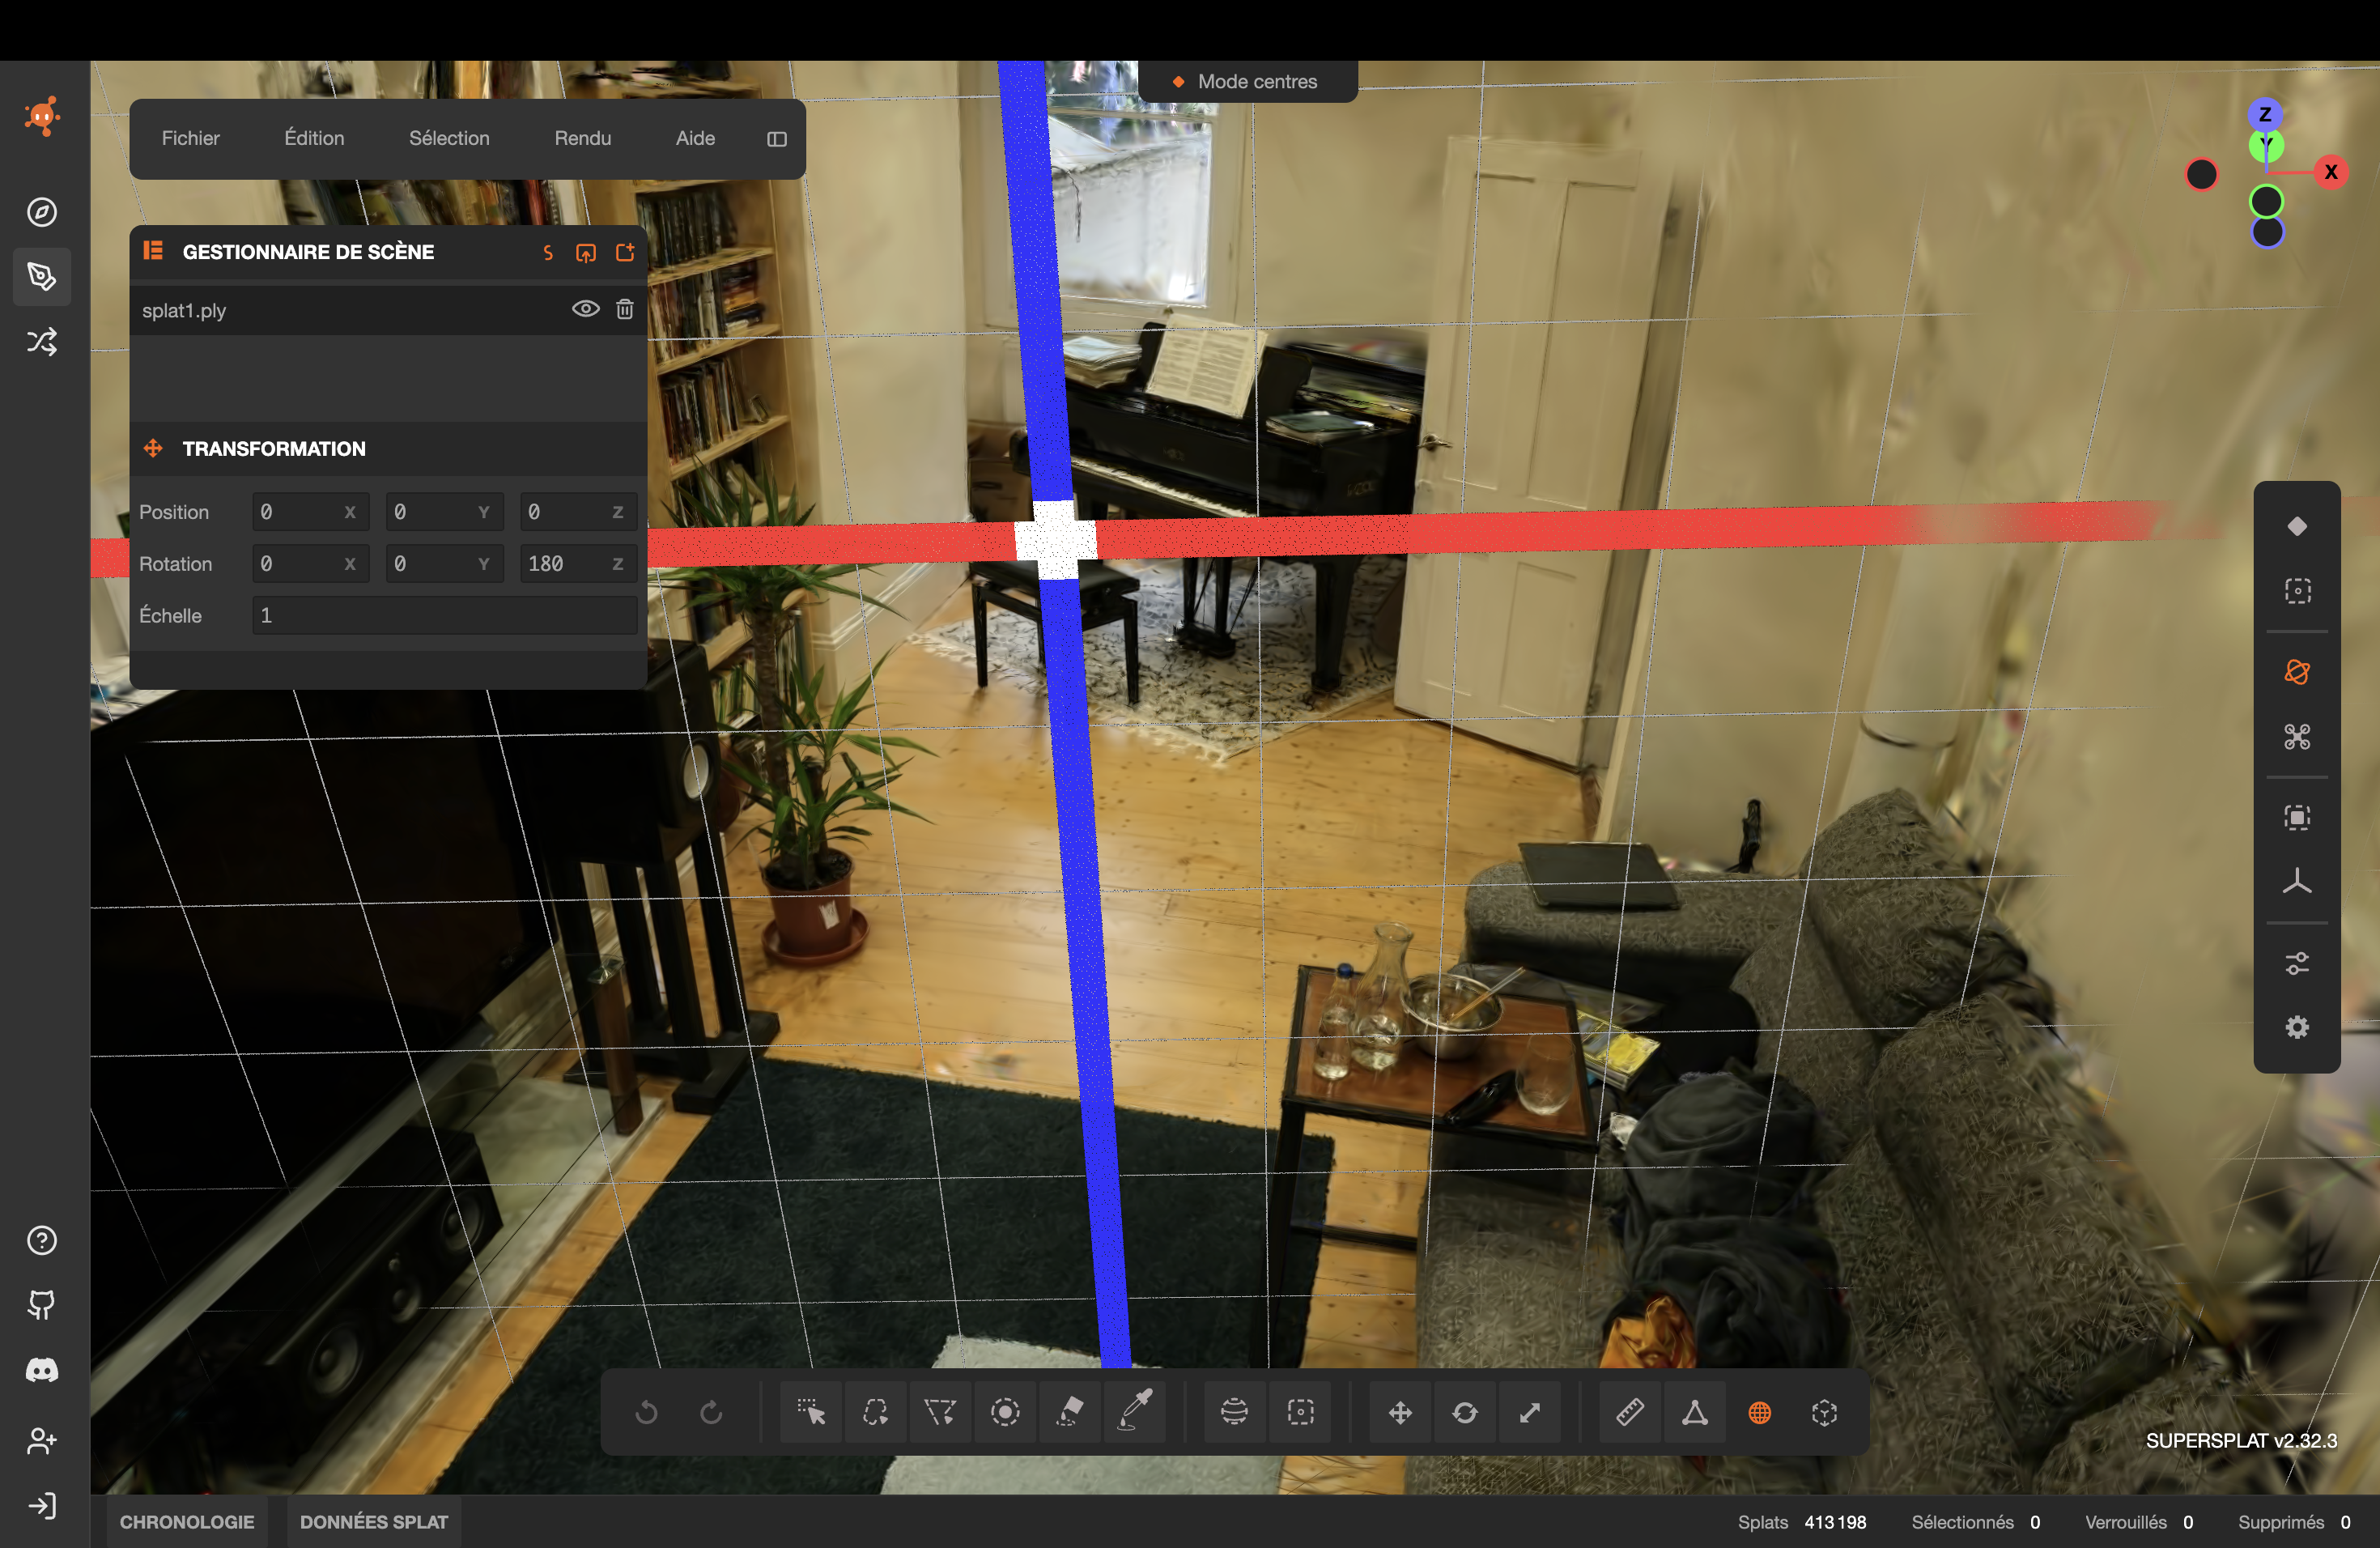
\includegraphics[width=0.8\linewidth]{images/scene3DGS.png}
    \caption{Visualisation de la scène 3D construite}, 
    \label{fig:scene3D}
\end{figure}

\begin{figure}[H]
    \centering
    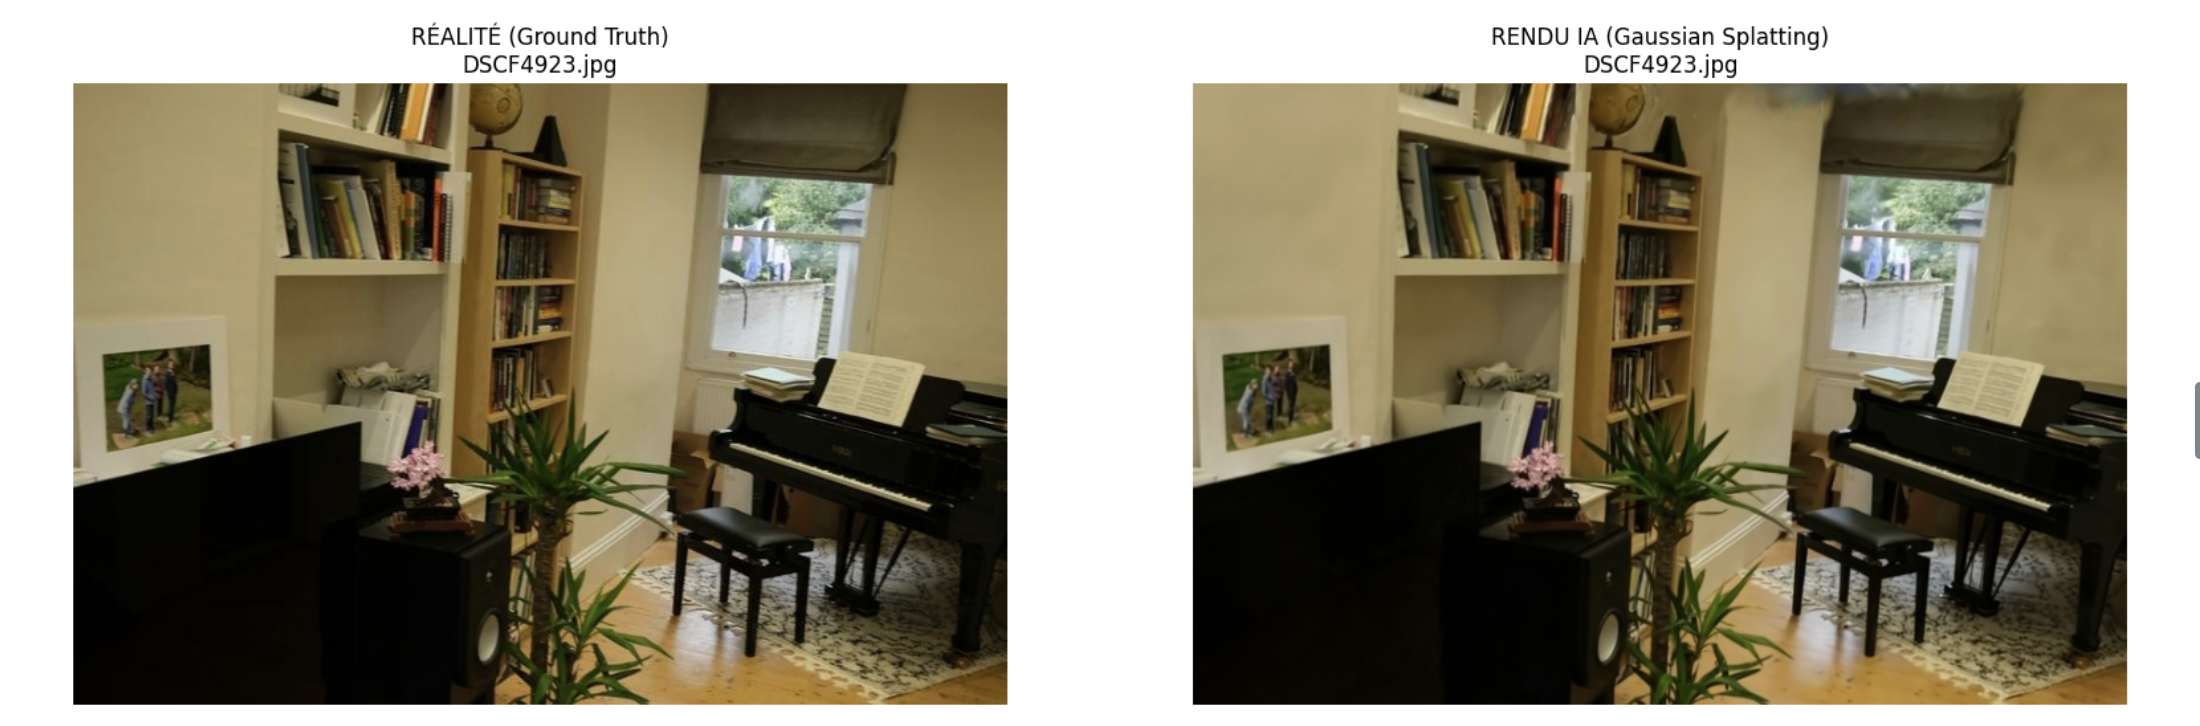
\includegraphics[width=1.2\linewidth]{images/rendu_vs_truth.png}
    \caption{Comparaison entre les images réelles (\textit{ground truth}) et les vues synthétisées par le modèle 3DGS (\textit{rendu}) sur la séquence \textit{room}.}
    \label{fig:rendu_vs_gt}
\end{figure}

\begin{figure}[H]
    \centering
    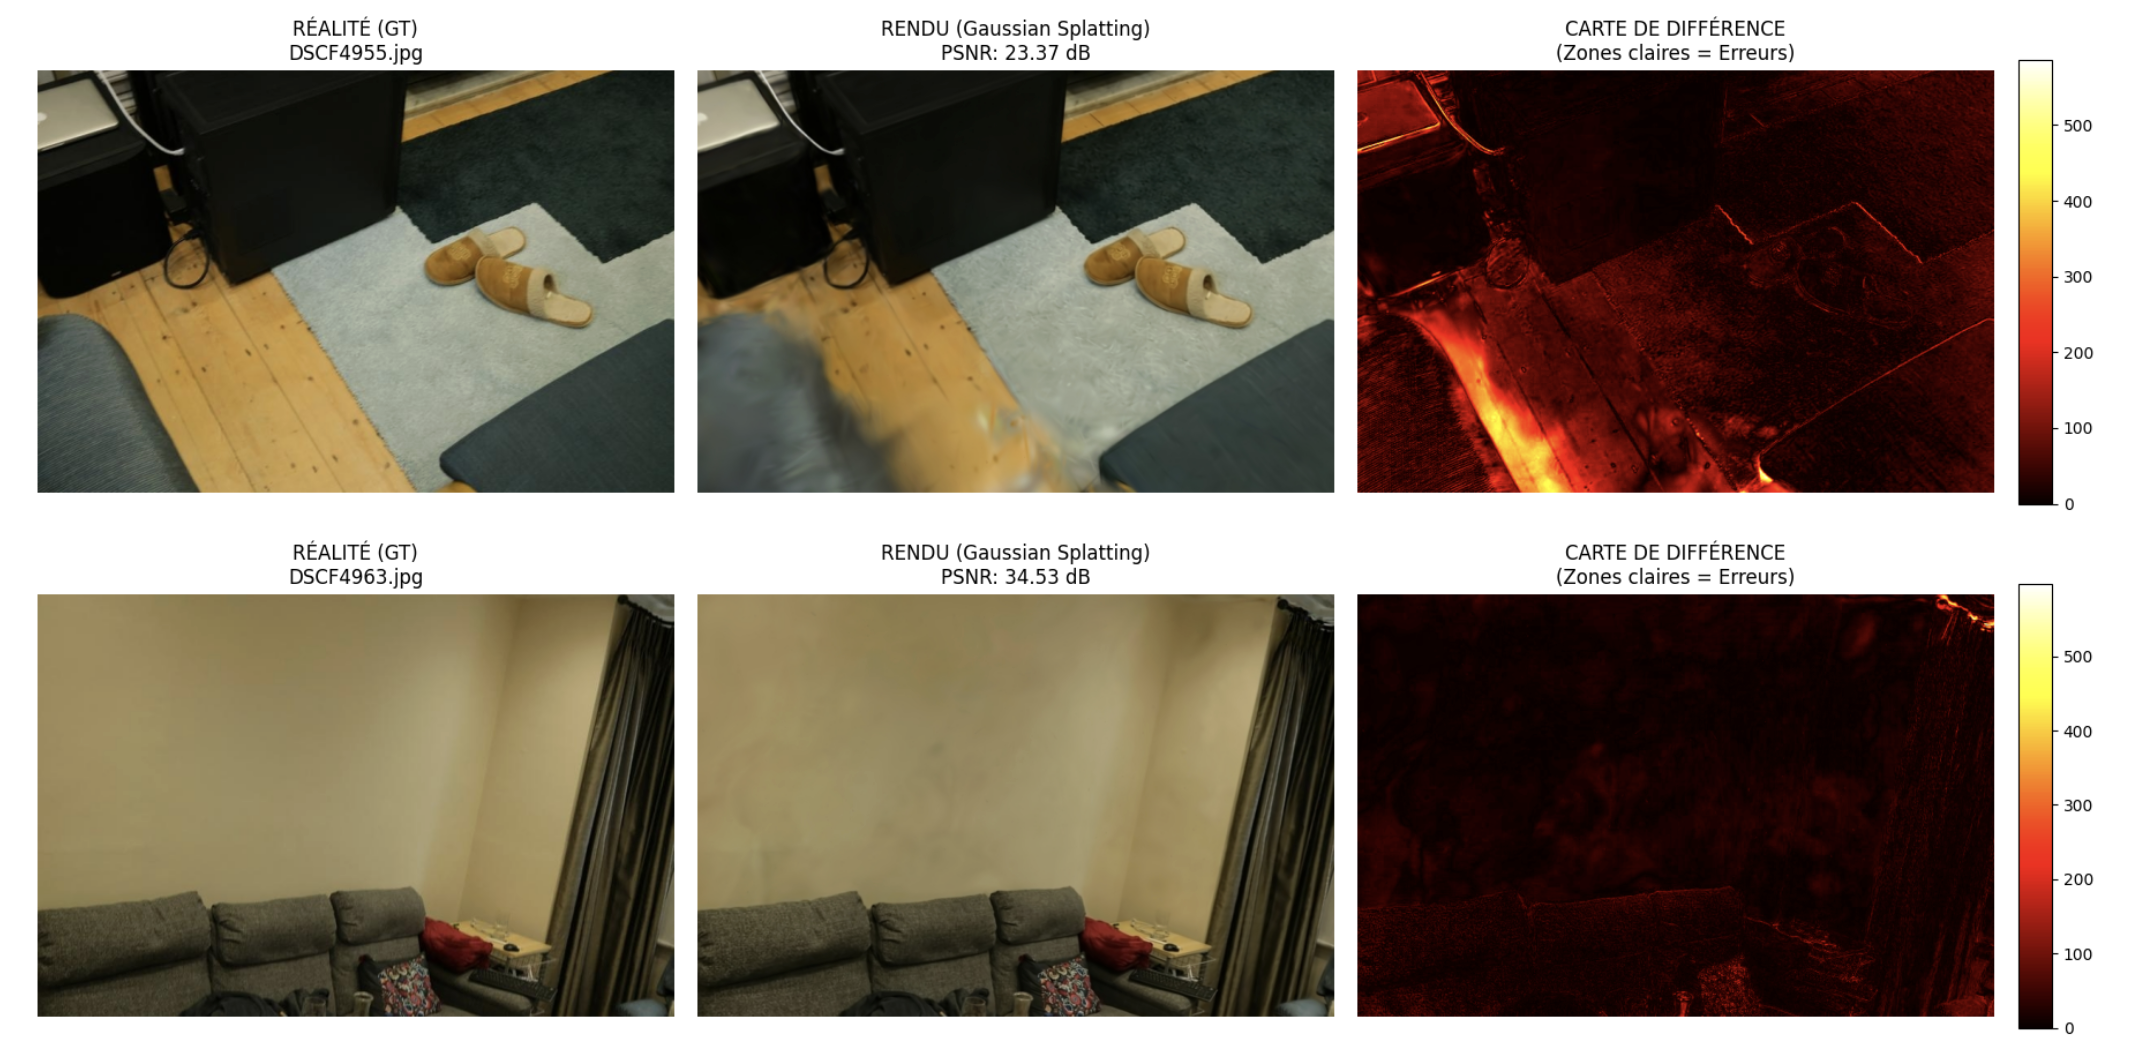
\includegraphics[width=0.95\linewidth]{images/diff_map.png}
    \caption{Comparaison entre les images réelles , les rendus 3DGS et les cartes de différence pixel à pixel}
    \label{fig:diff_map}
\end{figure}

\subsubsection*{Observations}

\begin{itemize}
    \item Dans la figure~\ref{fig:rendu_vs_gt} on voit que les rendus du modèle 3DGS sont globalement plus nets que les images réelles, ce phénomène peut s'expliquer par le fait que le 3DGS effectue une forme de régularisation implicite qui lisse les imperfections et le bruit des capteurs photographiques. Le modèle reconstruit les surfaces de manière lisse, agissant ainsi comme \textbf{un filtre de restauration}.
    \item Cependant, la Figure~\ref{fig:diff_map} révèle que certains rendus présentent des erreurs notables. Ces erreurs se concentrent principalement sur les zones à fort contraste et les bords d'objets, tandis que les surfaces lisses (murs, sol) sont très bien reconstituées.
\end{itemize}



\subsubsection*{Évaluation quantitative}

Le modèle est évalué sur l'ensemble de test à l'aide du PSNR. Un résultat 
de :

\begin{equation}
    \text{PSNR} = 31.49 \text{ dB}
    \label{eq:psnr}
\end{equation}

est obtenu, ce qui indique une reconstruction des couleurs très fidèle à la réalité. 


\subsection{Reproduction du pipeline de navigation visuelle (AI2-THOR)}
\label{sec:aithor}

Dans cette section, nous expliquant le pipeline de navigation visuelle par RL proposé précédemment par Zhu et al. \cite{ref10}, que nous reproduisons et validons avant de l'adapter à notre scène 3DGS.


\subsubsection*{Formulation de la politique}

L'approche standard de navigation visuelle consiste à apprendre une 
politique $\pi(a | s_t, u)$ où la cible est implicitement encodée dans 
les poids $u$ du réseau — un réseau par cible, nécessitant un 
ré-entraînement complet pour chaque nouvel objet cible.

L'originalité de l'approche de Zhu et al. est de donner la cible $g$ 
\textbf{explicitement en entrée} du réseau :

\begin{equation}
    a \sim \pi(s_t, g \mid u)
    \label{eq:policy_aithor}
\end{equation}

où $s_t$ est l'image courante (image RGB) et $g$ est l'image de la cible. 

Cette formulation permet de \textbf{régler le problème fondamental du RL et de généraliser à de nouvelles cibles} sans ré-entraîner le réseau, comme illustré dans la 
Figure~\ref{fig:approches}.

\begin{figure}[H]
    \centering
    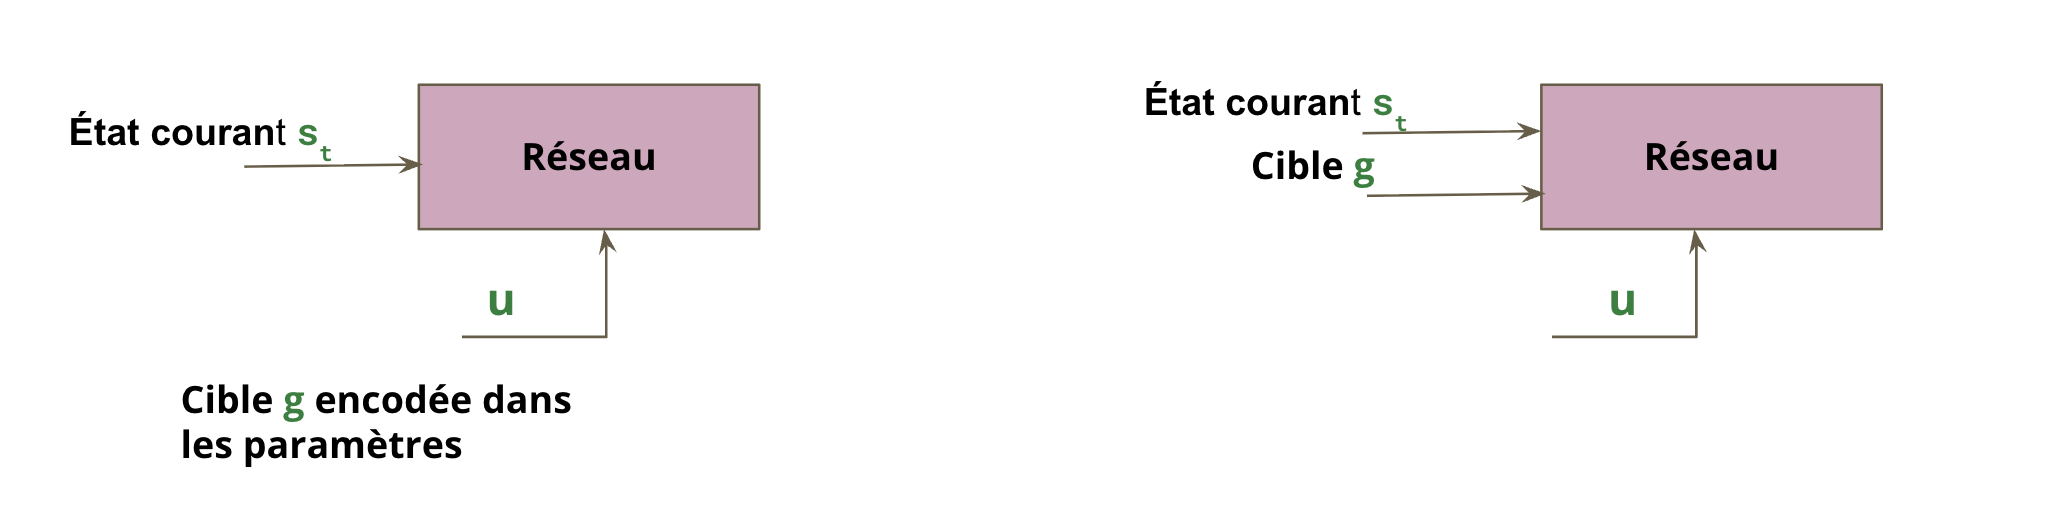
\includegraphics[width=1.0\linewidth]{images/approches.png}
    \caption{Comparaison entre l'approche standard  et l'approche de Zhu et al. \cite{ref10} }
    \label{fig:approches}
\end{figure}

\subsubsection*{Architecture du réseau}

Le réseau est une architecture \textbf{siamoise} composée de deux 
\textit{streams} parallèles partageant les mêmes poids, comme illustré 
dans la Figure~\ref{fig:archi_siamois} :

\begin{figure}[H]
\centering
\begin{tikzpicture}[
    node distance=1.2cm and 1.0cm,
    every node/.style={font=\small},
    box/.style={rectangle, rounded corners=3pt, draw, fill=#1, 
                minimum width=2.2cm, minimum height=1.2cm, align=center},
    arrow/.style={-{Stealth}, thick},
]

%--- Inputs ---
\node[box=blue!15] (obs) {\textbf{Observation} \\ $224\times224\times3$};
\node[box=blue!15, below=2cm of obs] (goal) {\textbf{Goal} \\ $224\times224\times3$};

%--- ResNet-50 ---
\node[box=orange!30, right=0.6cm of obs] (resnet1) {\textbf{ResNet-50} \\ 2048d};
\node[box=orange!30, right=0.6cm of goal] (resnet2) {\textbf{ResNet-50} \\ 2048d};

%--- W partagé ---
\node[draw, fill=white, minimum width=0.6cm, minimum height=0.6cm,
      font=\small\bfseries] (W) at ($(resnet1)!0.5!(resnet2)$) {W};

%--- FC ---
\node[box=pink!40, right=0.6cm of resnet1] (fc1) {fc \\ 512d};
\node[box=pink!40, right=0.6cm of resnet2] (fc2) {fc \\ 512d};

%--- Embedding Fusion ---
\node[box=green!20, minimum width=0.2cm, minimum height=4.7cm,
      right=0.6cm of fc1, yshift=-1.6cm] (fusion) 
      {\textbf{Embedding} \\ \textbf{Fusion} \\ \\ concat \\ 1024d \\ $\rightarrow$ 512d};

%--- Scene-Specific ---
\node[box=red!25, right=0.6cm of fusion] (scene) 
      {\textbf{Scene-} \\ \textbf{Specific} \\ \textbf{Layers}};

%--- Actor-Critic ---
\node[box=blue!30, right=0.8cm of scene] (ac) {\textbf{Actor-Critic}};

%--- Flèches ---
\draw[arrow] (obs) -- (resnet1);
\draw[arrow] (goal) -- (resnet2);
\draw[arrow] (resnet1) -- (fc1);
\draw[arrow] (resnet2) -- (fc2);
\draw[arrow] (fc1.east) -- (fusion.west |- fc1);
\draw[arrow] (fc2.east) -- (fusion.west |- fc2);
\draw[arrow] (fusion) -- (scene);
\draw[arrow] (scene) -- (ac);

%--- W double flèche ---
\draw[{Stealth}-{Stealth}, thick] (resnet1) -- (W);
\draw[{Stealth}-{Stealth}, thick] (W) -- (resnet2);

\end{tikzpicture}
\caption{Architecture du réseau siamois pour la navigation visuelle \cite{ref10}.}
\label{fig:archi_siamois}
\end{figure}

\vspace{1cm}
Le réseau se compose de deux types de couches :

\begin{itemize}[noitemsep, topsep=4pt]
    \item \textbf{Couches siamoises génériques} (\textit{Generic Siamese 
    Layers}) : poids $W$ partagés entre les deux streams pour projeter 
    $s_t$ et $g$ dans le même espace d'embedding de 512 dimensions. 
    Les relations géométriques entre les deux embeddings sont ainsi 
    préservées — lorsque l'agent se trouve devant la cible, les deux 
    embeddings sont proches, ainsi le réseau produit l'action 
    \texttt{stop}.
    \item \textbf{Couches spécifiques à la scène} (\textit{Scene-specific 
    Layers}) : une par scène, capturant les caractéristiques propres à 
    chaque environnement (disposition des pièces, arrangement des objets).
\end{itemize}

\subsubsection*{Détection de la cible et entraînement}

La navigation est \textbf{discrète} : l'agent se déplace sur une grille 
de positions prédéfinies, stockées dans un fichier HDF5. À chaque pas 
de temps, le code consulte un graphe de transitions (\texttt{transition\_graph}) 
pour déterminer la nouvelle position de l'agent. L'agent dispose de 
4 actions : \texttt{MoveForward}, \texttt{RotateRight}, 
\texttt{RotateLeft} et \texttt{MoveBackward}.

\begin{figure}[H]
    \centering
    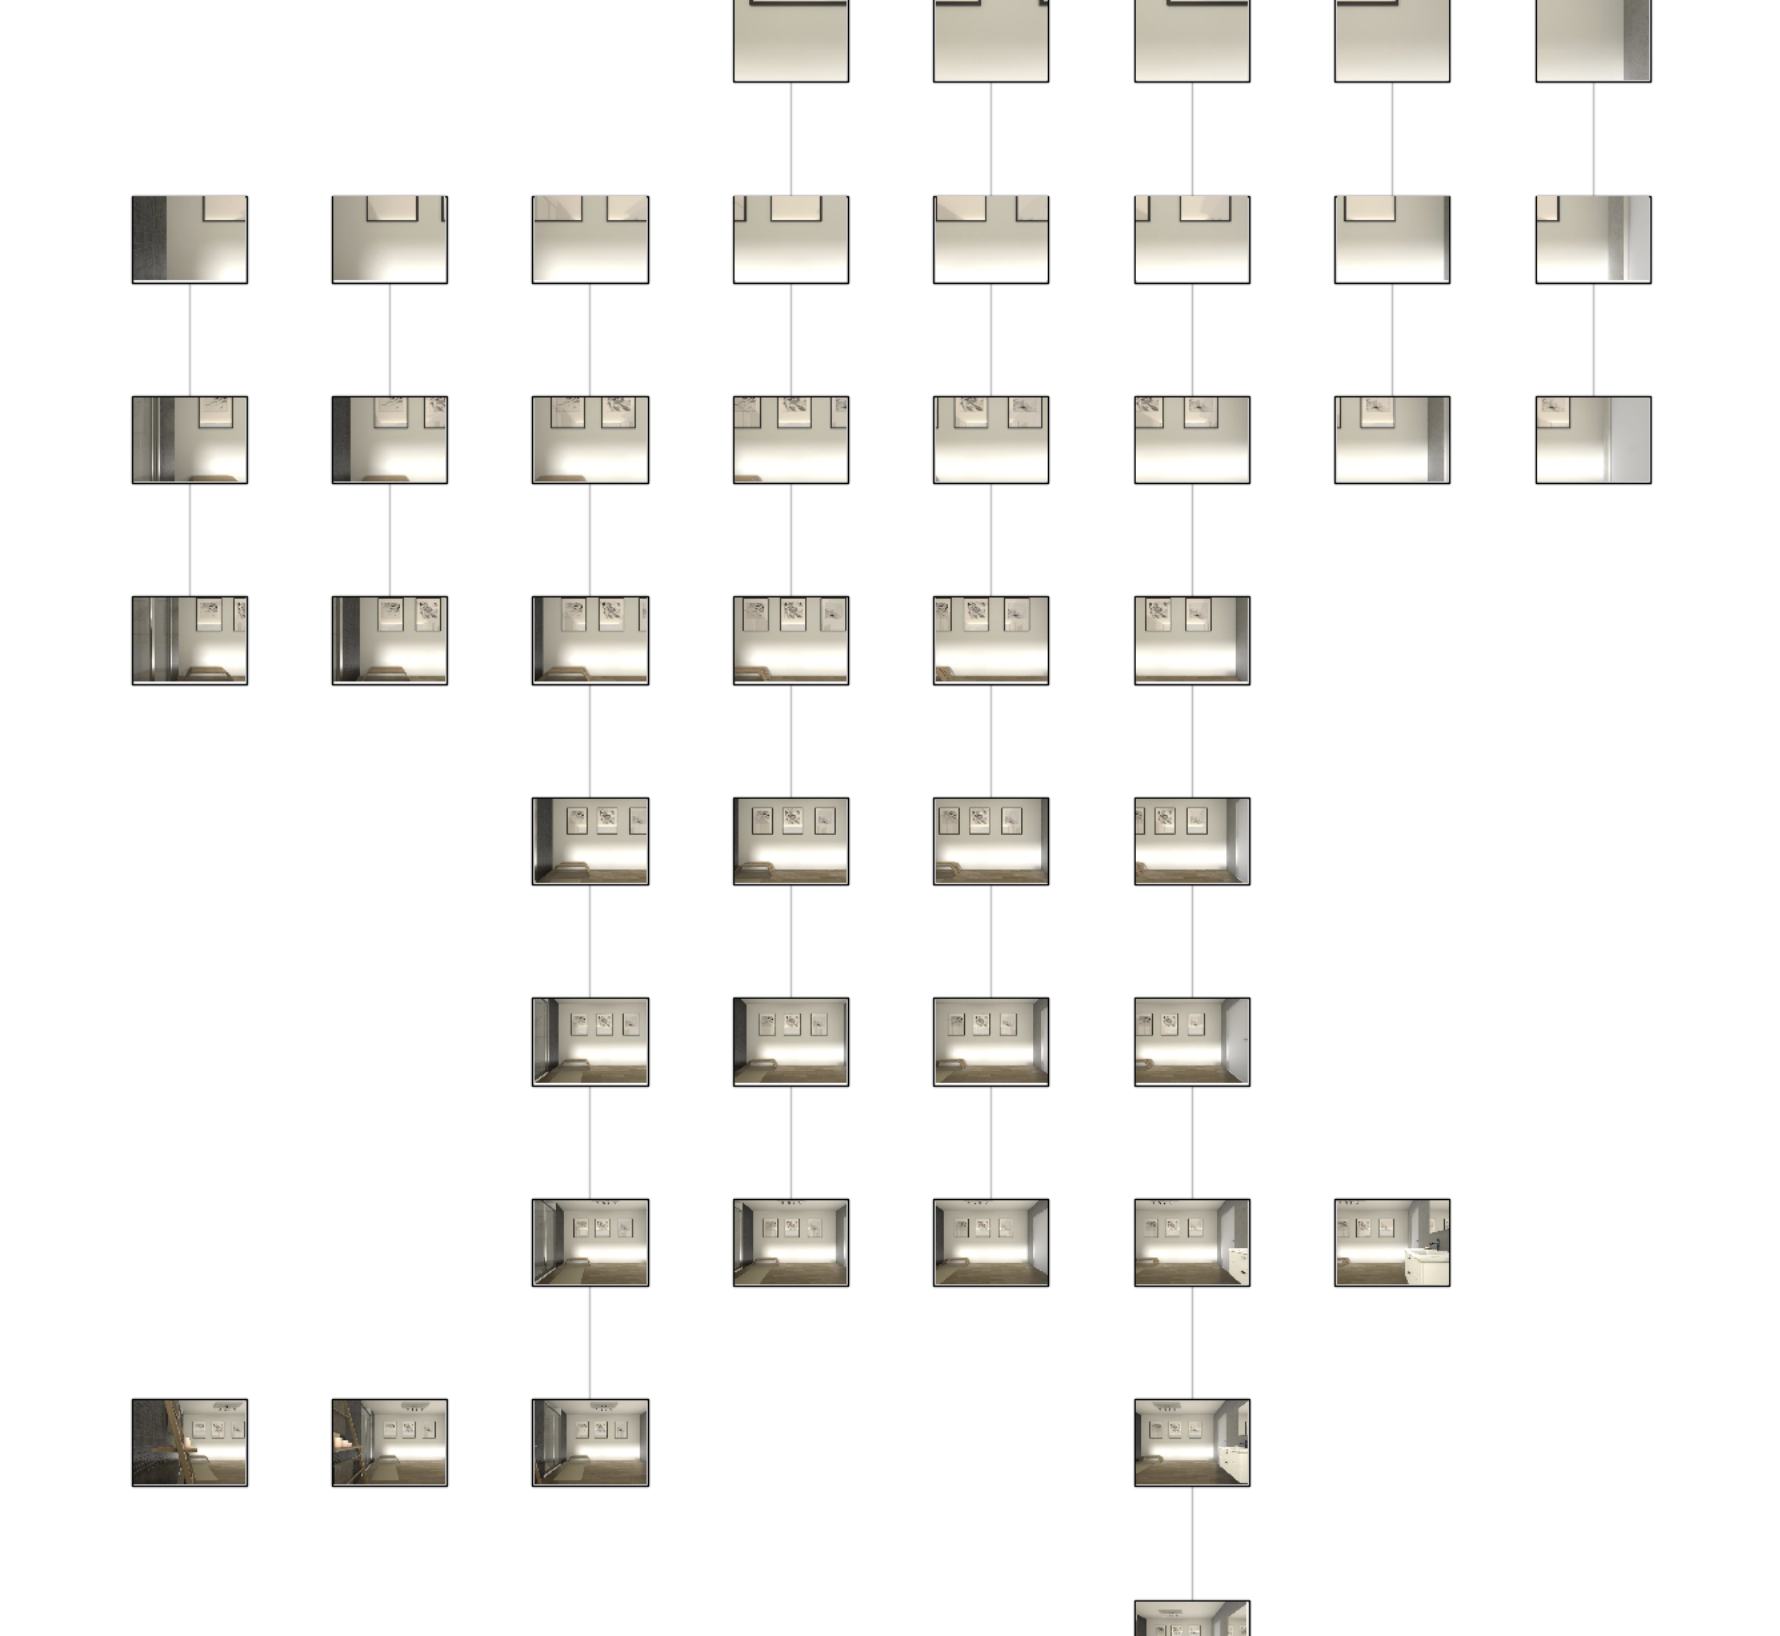
\includegraphics[width=0.8\linewidth]{images/graphe-aithor.png}
    \caption{Exemple de graphe de navigation AI2-THOR original (\texttt{data/bathroom\_02.h5}) — 45 nœuds, yaw = 0°.}
    \label{fig:graphe-aithor}
\end{figure}

L'épisode est considéré comme réussi uniquement lorsque l'agent atteint 
\textbf{exactement} la position de la cible (\texttt{terminal\_state\_id}). 
La fonction de récompense est définie comme suit :

\begin{equation}
    r_t = \begin{cases}
        +10 & \text{si la nouvelle position} = \text{position cible} \\
        -0.1 & \text{en cas de collision} \\
        -0.01 & \text{à chaque pas normal}
    \end{cases}
    \label{eq:reward_aithor}
\end{equation}

L'agent ne sait pas immédiatement si un pas est bon ou mauvais — la 
récompense est identique ($-0.01$) dans les deux cas. C'est le 
\textbf{Critique} qui apprend progressivement à distinguer les bonnes 
positions des mauvaises, via l'erreur temporelle TD :

\begin{equation}
    \delta_t = R_t - V(s_t)
    \label{eq:td_error}
\end{equation}

où $R_t$ est la somme des récompenses futures réellement obtenues et 
$V(s_t)$ est l'estimation du Critique. Cette différence permet au 
Critique de corriger ses estimations au fil des épisodes — il apprend 
que certaines positions mènent souvent à $+10$ rapidement (bonnes 
positions) et d'autres rarement (mauvaises positions). L'Acteur utilise 
ensuite ces estimations pour choisir les actions menant vers les bonnes 
positions. C'est donc uniquement après des milliers d'épisodes que le 
système apprend à naviguer efficacement.

L'ensemble du réseau est entraîné de bout en bout (\textit{end-to-end}) 
via ce unique signal de récompense, sans \textit{feature engineering} 
manuel, sans \textit{feature matching} entre frames, et sans 
reconstruction 3D explicite de l'environnement.


\paragraph{NB:}

Les scènes AI2-THOR sont téléchargées depuis le serveur de Stanford 
Vision Lab \footnote{\url{http://vision.stanford.edu/yukezhu/thor_v1_scene_dumps.zip}} 
et fournies sous forme de fichiers HDF5 (\texttt{bathroom\_02.h5}, 
\texttt{bedroom\_04.h5},
\texttt{kitchen\_02.h5},
\texttt{living\_room\_08.h5}), chacune contenant le graphe de navigation, les images RGB et les features ResNet-50 associées à chaque état.

\subsubsection*{Résultats et comparaison}

Après l'entraînement complet sur 100 millions de frames avec 100 threads parallèles, l'évaluation sur 100 épisodes par cible donne les longueurs moyennes de trajectoire suivantes :



\begin{table}[H]
\centering
\footnotesize
\renewcommand{\arraystretch}{1.3}
\begin{tabular}{|l|c|}
\hline
\rowcolor{gray!20}
\textbf{Scène} & \textbf{Longueur moyenne (pas)} \\
\hline
\texttt{bathroom\_02}     & 7.8  \\
\texttt{bedroom\_04}      & 15.1 \\
\texttt{living\_room\_08} & 16.7 \\
\texttt{kitchen\_02}      & 21.6 \\
\hline
\rowcolor{blue!15}
\textbf{Moyenne (notre réimplémentation)} & \textbf{15.3} \\
\hline
\rowcolor{orange!20}
\textbf{Moyenne article} \cite{ref10}     & \textbf{210.7} \\
\hline
\end{tabular}
\caption{Longueurs moyennes de trajectoire obtenues sur les 4 scènes et 20 cibles.}
\label{tab:aithor_results}
\end{table}


\begin{figure}[H]
    \centering
    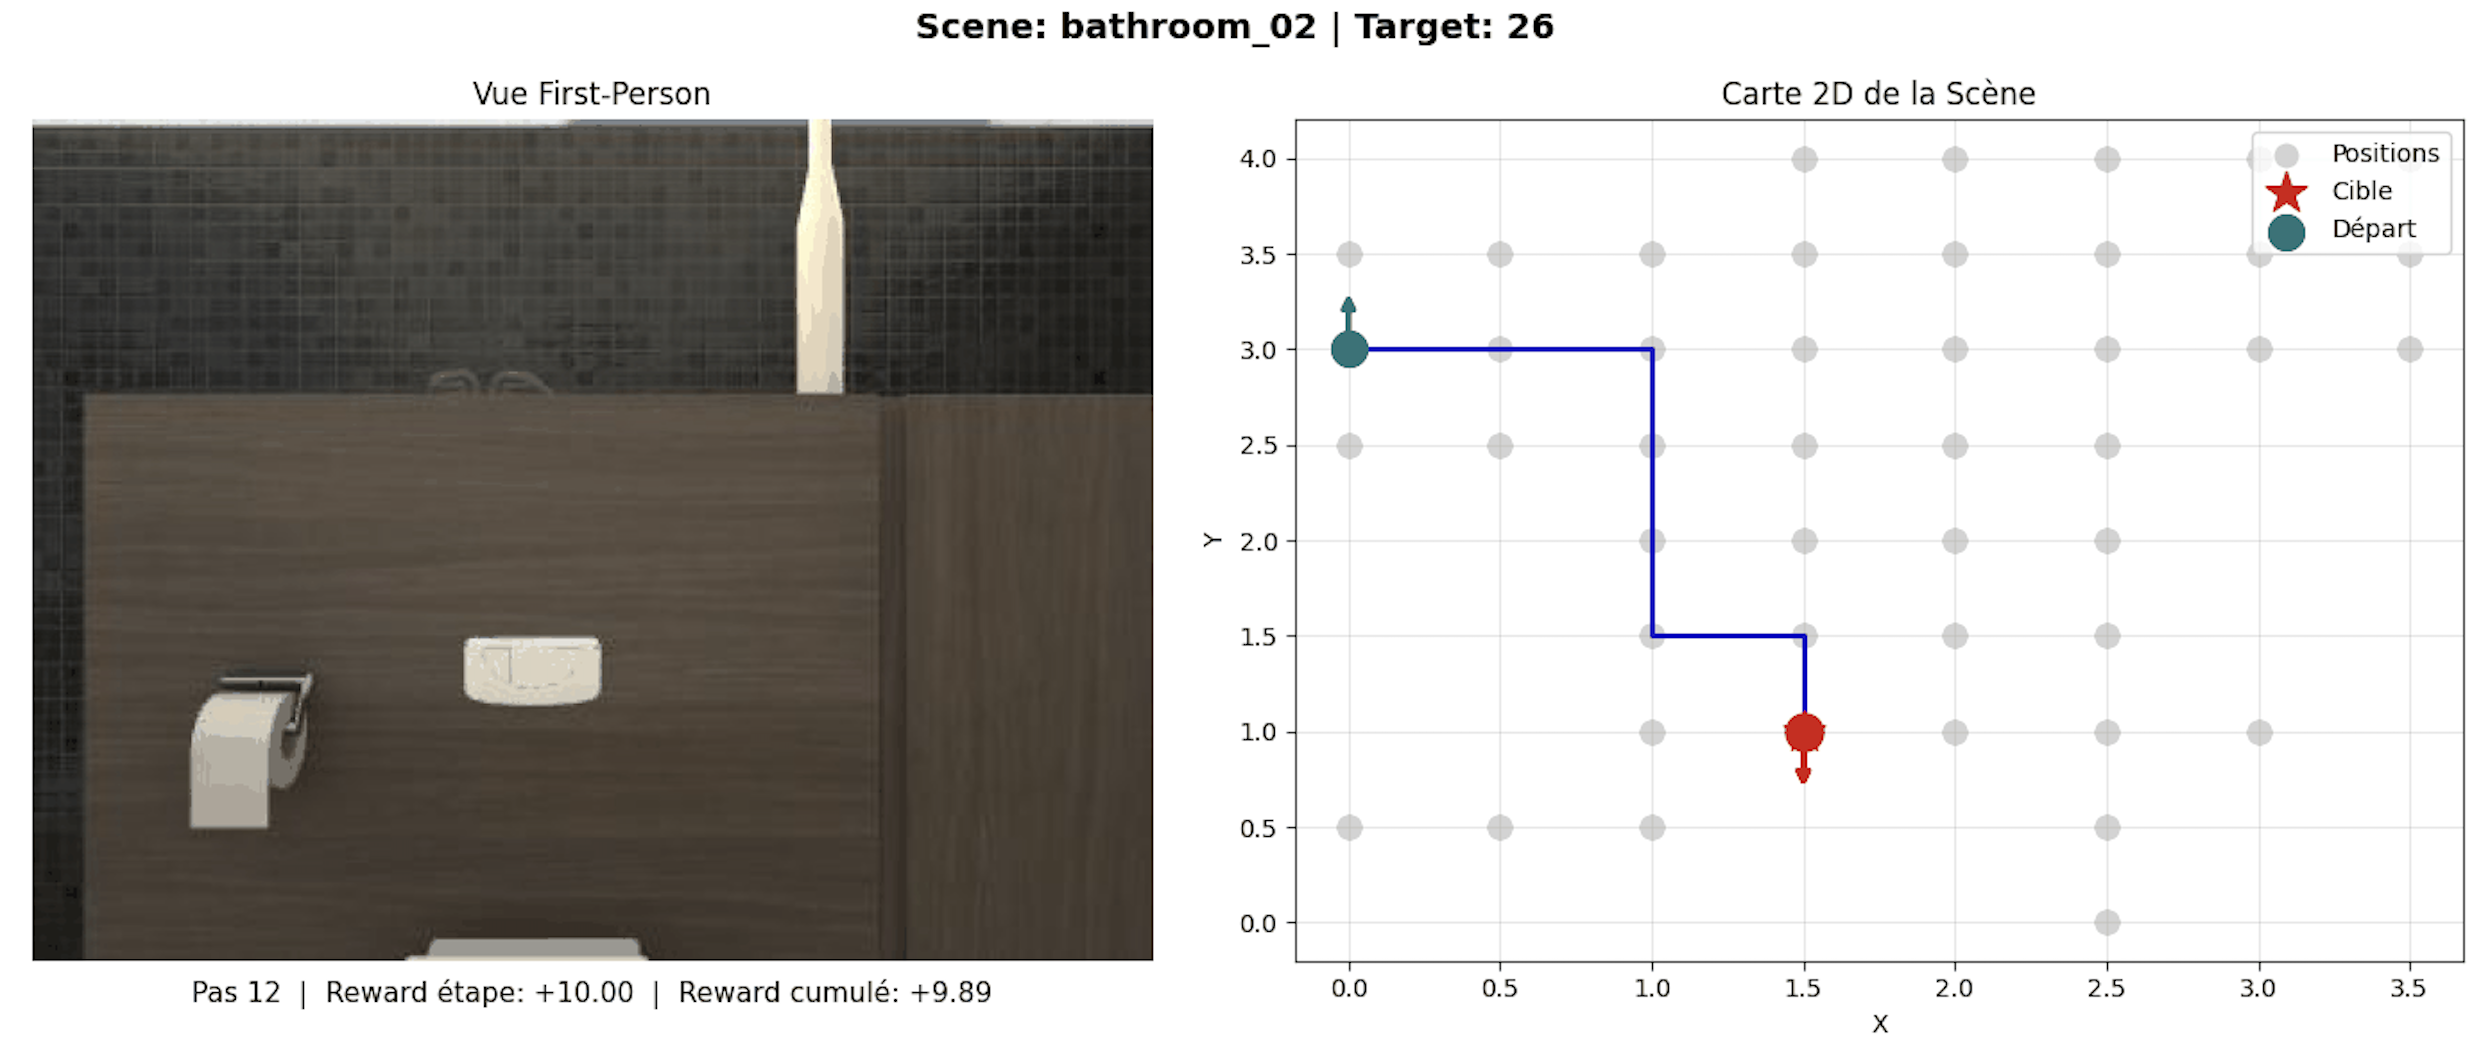
\includegraphics[width=0.9\linewidth]{images/animation_aithor.png}
    \caption{Exemple de navigation de l'agent A3C sur la scène \texttt{bathroom\_02} (cible 26)}
    \label{fig:animation_aithor}
\end{figure}

\subsubsection*{Remarques}
\begin{itemize}
    \item L'article original de Zhu et al. \cite{ref10} rapporte, dans sa Table I, 
    une longueur moyenne de trajectoire de 210.7 pas pour leur modèle final 
    (\textit{Target-driven final}), contre 15.3 pas pour notre 
    réimplémentation. Leurs résultats sont obtenus sur un ensemble de 100 
    cibles échantillonnées aléatoirement parmi 20 scènes intérieures. En 
    revanche, le code source mis à disposition publiquement par les auteurs 
    ne contient que 4 scènes (une par catégorie : salle de bain, chambre, 
    cuisine, salon), correspondant exactement aux scènes utilisées dans cette 
    réimplémentation. Une comparaison numérique directe n'est donc pas 
    rigoureusement valide, le sous-ensemble réduit utilisé ici facilitant 
    mécaniquement la convergence de l'agent du fait d'un espace de tâches 
    beaucoup plus restreint.
    \item Une comparaison plus appropriée consiste à situer nos résultats par 
    rapport à la borne théorique du plus court chemin (17.6 pas) 
    \cite{ref10}. La longueur moyenne obtenue sur les quatre scènes est de 15.3 pas, se 
    situe bien dans cet ordre de grandeur, ce qui montre la validité et la bonne convergence de la politique apprise.
\end{itemize}









\subsection{Construction du graphe 3DGS et entraînement sur room}
\label{sec:graphe_room}



Dans cette section, nous adaptons le pipeline de navigation visuelle développé précédemment pour AI2-THOR,  à la scène \textit{room} reconstruite par 3DGS. Cette partie  comprend deux grandes étapes  : la construction d'un graphe de navigation discret, et l'entraînement de l'agent A3C sur ce graphe.



\subsubsection{Construction du graphe de navigation}

D'après les poses extraites du fichier COLMAP , et du fichier \texttt{splat.ply}(section~\ref{sec:resulats1}). La construction suit le pipeline suivant : 

\vspace{0.4cm}
\textbf{1. Extraction des poses COLMAP} : 

les 311 poses de caméra sont lues depuis les fichiers binaires COLMAP 
(\texttt{cameras.bin}, \texttt{images.bin}). Pour chaque pose, on extrait la position 3D du centre de la caméra $\mathbf{C} = -\mathbf{R}^\top \mathbf{t}$ et le vecteur vertical  réel de la scène \texttt{up\_world}, calculé comme la moyenne des vecteurs $-\mathbf{R}[1,:]$ sur toutes les images. 

\begin{figure}[H]
    \centering
    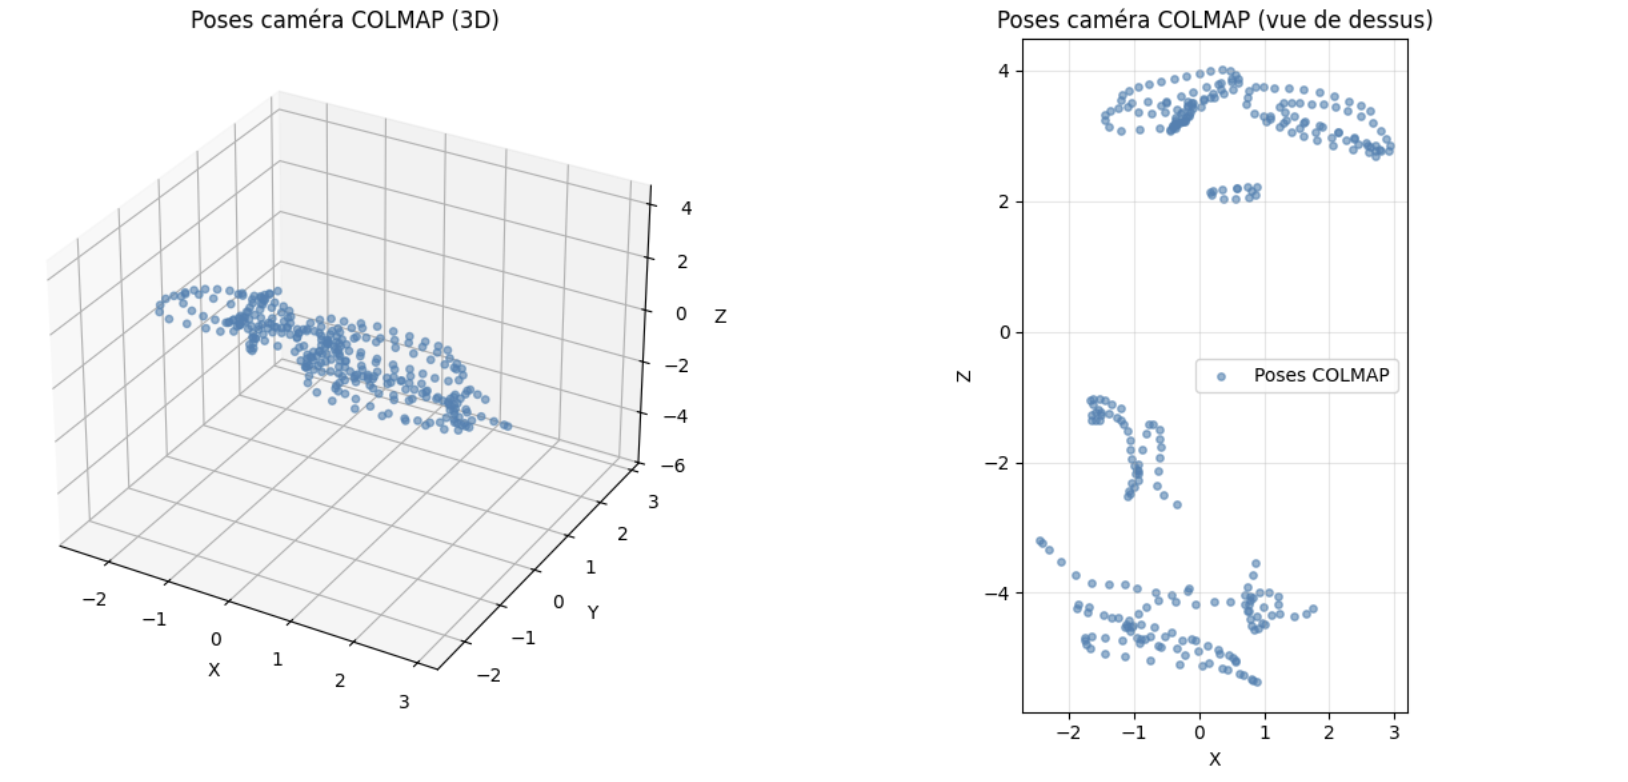
\includegraphics[width=1\linewidth]{images/poses-cam.png}
    \caption{Disposition des poses caméra dans le scène room}
    \label{fig:grille_room}
\end{figure}

On constate que les positions des caméras forment trois clusters séparés plutôt qu'une grille uniforme, comme illustré dans la 
Figure~\ref{fig:grille_room}. 
Ceci est dû au fait que: dans une scène à 360°, les caméras tournent autour du centre de la pièce à hauteur humaine, et non à hauteur de robot au niveau du sol.

\vspace{0.4cm}
\textbf{2. Projection dans le plan du sol et construction de l'enveloppe convexe} :


 les centres de caméra sont projetés dans le plan orthogonal à \texttt{up\_world} via deux axes horizontaux \texttt{axis\_u} et \texttt{axis\_v}, définissant un repère 2D adapté à la géométrie réelle de la scène. Ensuite, une enveloppe convexe (\textit{Convex Hull}) est calculée sur l'ensemble des 
projections 2D des poses COLMAP, définissant la zone navigable de la scène.

\begin{figure}[H]
    \centering
    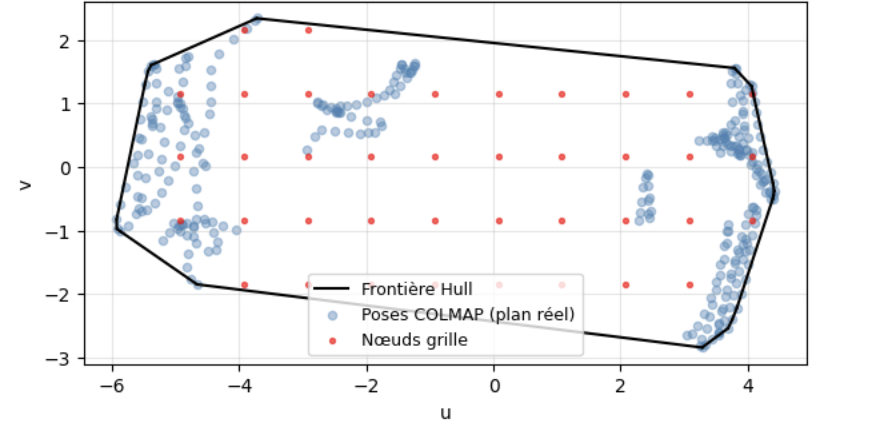
\includegraphics[width=0.8\linewidth]{images/enveloppe.png}
    \caption{Enveloppe convexe des poses COLMAP et grille de navigation}
    \label{fig:enveloppe-convexe}
\end{figure}


une grille uniforme de pas $\Delta = 1$ m est générée à l'intérieur de l'enveloppe convexe. Chaque nœud de la grille est associé à 4 orientations discrètes (yaw = 0°, 90°, 180°, 270°), produisant un total de $N_{\text{nodes}} \times 4$ états.

\vspace{0.4cm}
\textbf{3. Rendu des vues synthétiques} : 

pour chaque état (position, orientation), une vue est synthétisée via le renderer gsplat à partir du fichier \texttt{.ply} entraîné (section~\ref{sec:resulats1}). La chaîne de conversion des poses suit : repère COLMAP $\rightarrow$ repère OpenGL $\rightarrow$ transformation Nerfstudio (matrice \texttt{dataparser\_transforms.json} + facteurd'échelle $s = 0.172$) $\rightarrow$ matrice de vue gsplat.

\begin{figure}[H]
    \centering
    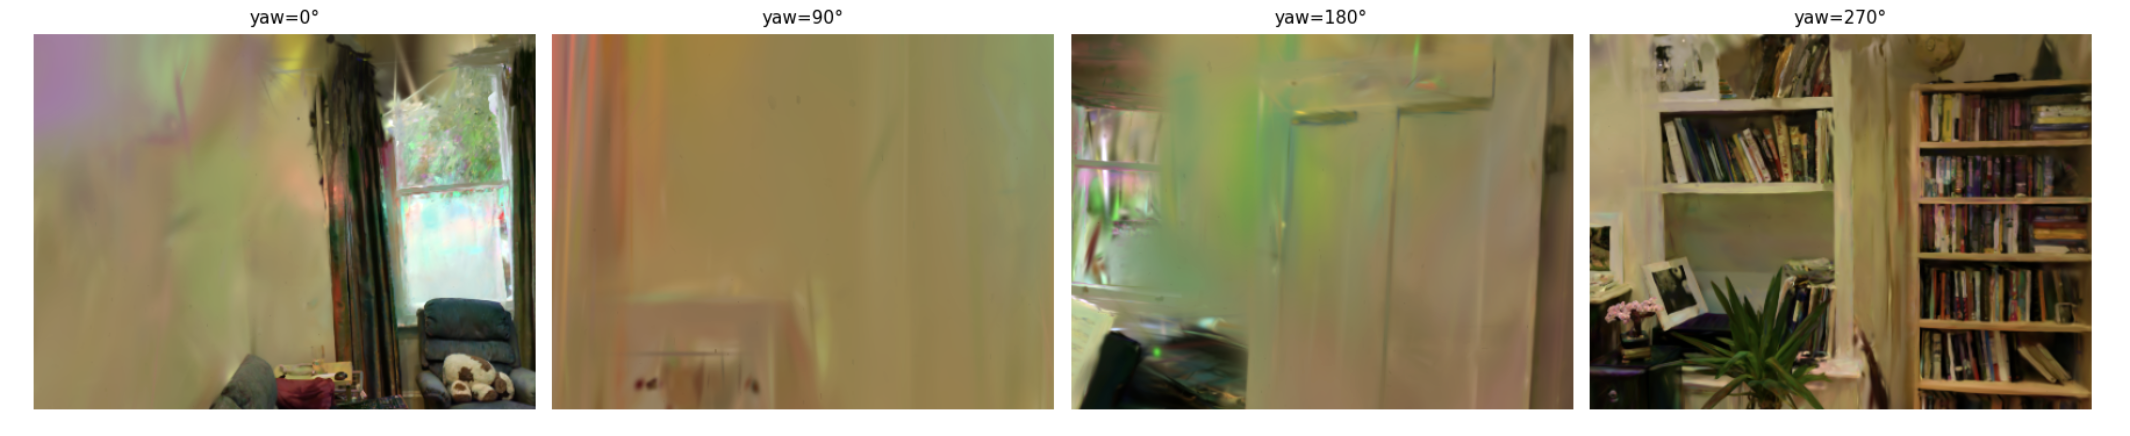
\includegraphics[width=1\linewidth]{images/rednu.png}
    \caption{Vues synthétisées par le renderer 3DGS depuis la position $(u = -3.93,\ v = 2.19)$ pour les quatre orientations cardinales (yaw = 0°, 90°, 180°, 270°)}
    \label{fig:rendu}
\end{figure}

\textbf{4. Extraction des features ResNet-50} :

pour chaque état, les features visuelles sont extraites via un encodeur ResNet-50 pré-entraîné sur ImageNet (gelé), en appliquant un \textit{10-crop} et en moyennant les 10 vecteurs de 2048 dimensions obtenus, produisant un vecteur final de dimension $(1, 2048)$.

\vspace{2cm}
\textbf{5. Génération du fichier HDF5} : 

le graphe de navigation, les features ResNet-50, les distances du plus court chemin (\textit{shortest path distance}) et les métadonnées sont sauvegardés dans un fichier \texttt{scene\_3dgs.h5} compatible avec le framework  ICRA 2017 ~\ref{fig:graphe-aithor}.


\begin{figure}[H]
    \centering
    \begin{subfigure}{0.48\textwidth}
        \centering
        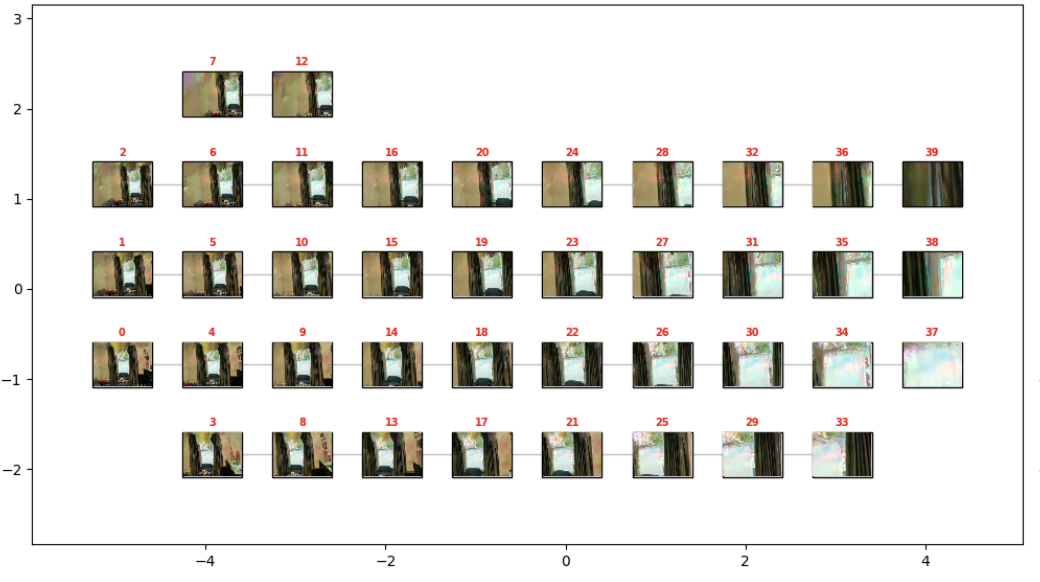
\includegraphics[width=\linewidth]{images/yaw0.png}
        \caption{yaw = 0°}
    \end{subfigure}
    \hfill
    \begin{subfigure}{0.48\textwidth}
        \centering
        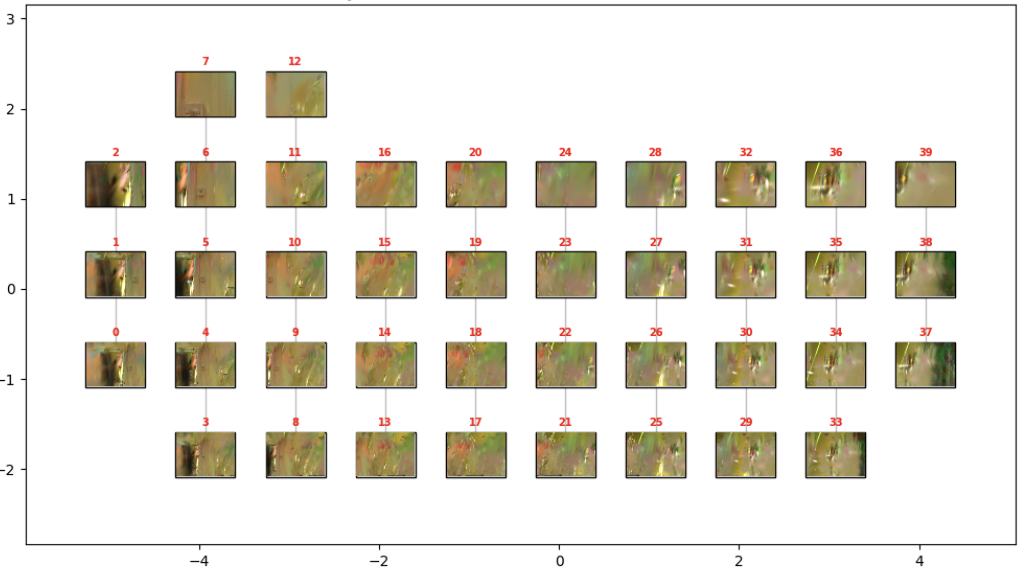
\includegraphics[width=\linewidth]{images/yaw90.png}
        \caption{yaw = 90°}
    \end{subfigure}
    
    \vspace{0.3cm}
    
    \begin{subfigure}{0.48\textwidth}
        \centering
        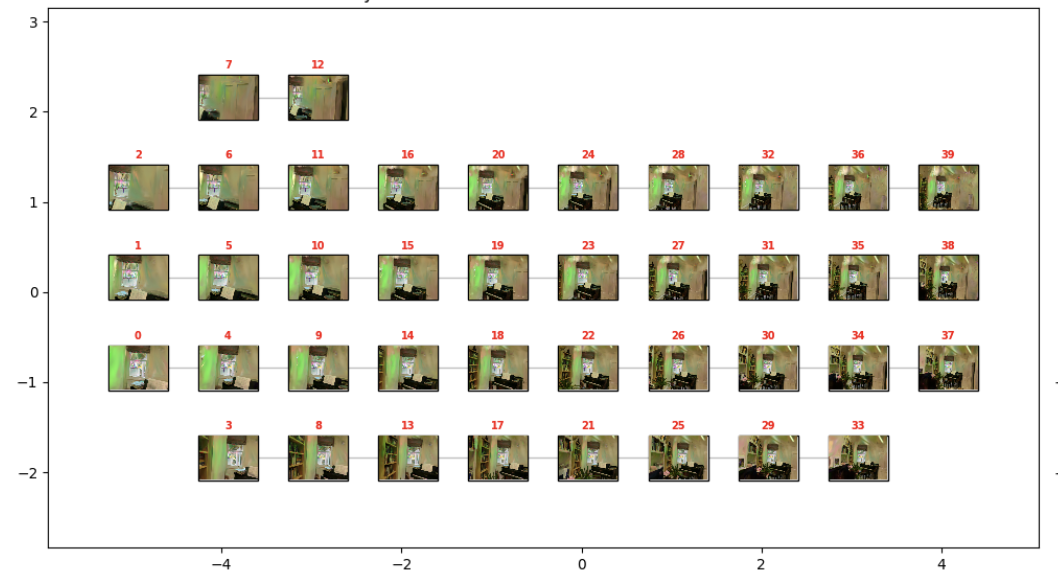
\includegraphics[width=\linewidth]{images/yaw180.png}
        \caption{yaw = 180°}
    \end{subfigure}
    \hfill
    \begin{subfigure}{0.48\textwidth}
        \centering
        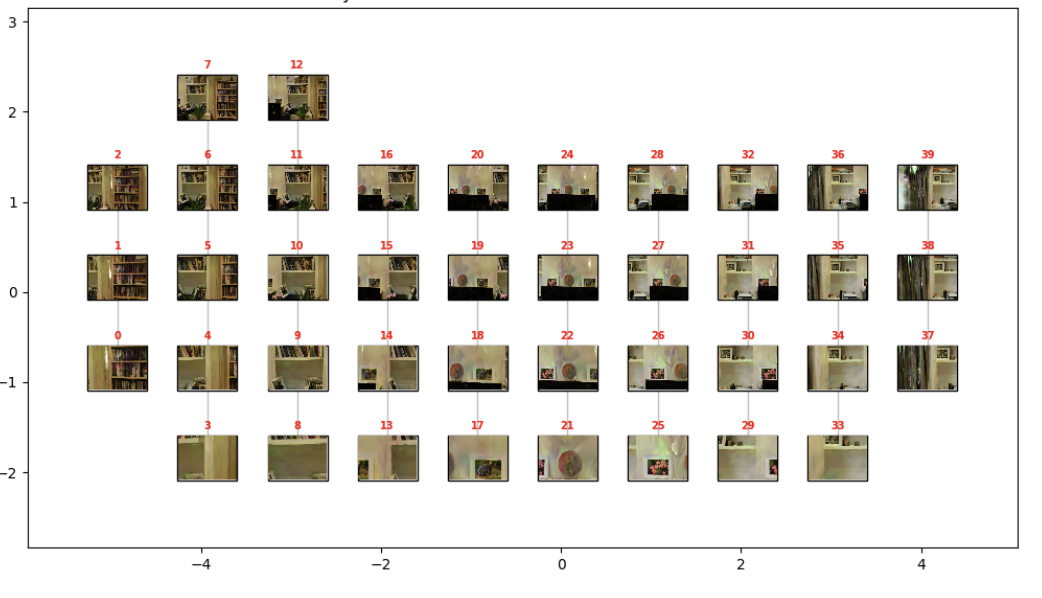
\includegraphics[width=\linewidth]{images/yaw270.png}
        \caption{yaw = 270°}
    \end{subfigure}
    
    \caption{Graphes de navigation par le render 3DGS  pour les quatre orientations cardinales 
    (yaw = 0°, 90°, 180°, 270°).}
    \label{fig:4_orientations}
\end{figure}

Le fichier HDF5 final contient les données suivantes :

\begin{table}[H]
\centering
\footnotesize
\renewcommand{\arraystretch}{1.3}
\begin{tabular}{|l|l|l|}
\hline
\rowcolor{gray!20}
\textbf{Clé} & \textbf{Forme} & \textbf{Description} \\
\hline
\texttt{graph} & $(N, 4)$ & Graphe de transitions (4 actions) \\
\texttt{resnet\_feature} & $(N, 1, 2048)$ & Features ResNet-50 \\
\texttt{shortest\_path\_distance} & $(N, N)$ & Distances du plus court chemin \\
\texttt{location} & $(N, 2)$ & Positions 2D dans le plan du sol \\
\texttt{poses\_names} & $(N,)$ & Identifiants des états \\
\hline
\end{tabular}
\caption{Structure du fichier HDF5 \texttt{scene\_3dgs.h5} généré pour 
la scène \textit{room}.}
\label{tab:hdf5_structure}
\end{table}

\subsubsection*{Entraînement A3C sur la scène \textit{room}}

L'agent A3C est entraîné sur le graphe de navigation 3DGS en suivant 
le même protocole que pour les scènes AI2-THOR, avec les adaptations 
suivantes :

\begin{itemize}[noitemsep, topsep=4pt]
    \item \textbf{Scène} : \texttt{room} (scène unique)
    \item \textbf{Cibles} : 5 états cibles fixes — états 
    \texttt{24, 60, 120, 108, 48}
    \item \textbf{Fonction de récompense} : identique à 
    \eqref{eq:reward_aithor} — $+10$ à la cible, $-0.1$ en collision, 
    $-0.01$ par pas
\end{itemize}

\subsubsection*{Résultats}




Le Tableau~\ref{tab:room_results} présente les résultats obtenus après 
10 millions frames d'entraînement sur la scène \textit{room}, pour les 
5 cibles sélectionnées.

\begin{table}[H]
\centering
\footnotesize
\renewcommand{\arraystretch}{1.3}
\begin{tabular}{|l|c|c|c|}
\hline
\rowcolor{gray!20}
\textbf{Cible} & \textbf{Reward moyen} & 
\textbf{Longueur moyenne (pas)} & \textbf{Collisions} \\
\hline
\texttt{\#24}  & 9.90 & 10.44 & 0.01 \\
\texttt{\#48}  & 9.92 & 8.78  & 0.06 \\
\texttt{\#60}  & 9.91 & 9.17  & 0.07 \\
\texttt{\#108} & 9.93 & 7.21  & 0.06 \\
\texttt{\#120} & 9.92 & 7.86  & 0.11 \\
\hline
\rowcolor{blue!15}
\textbf{Moyenne} & \textbf{9.92} & \textbf{8.69} & \textbf{0.06} \\
\hline
\end{tabular}
\caption{Résultats de l'agent A3C sur la scène \textit{room} 3DGS 
après 500\,000 frames d'entraînement (5 cibles).}
\label{tab:room_results}
\end{table}

\begin{figure}[H]
    \centering
    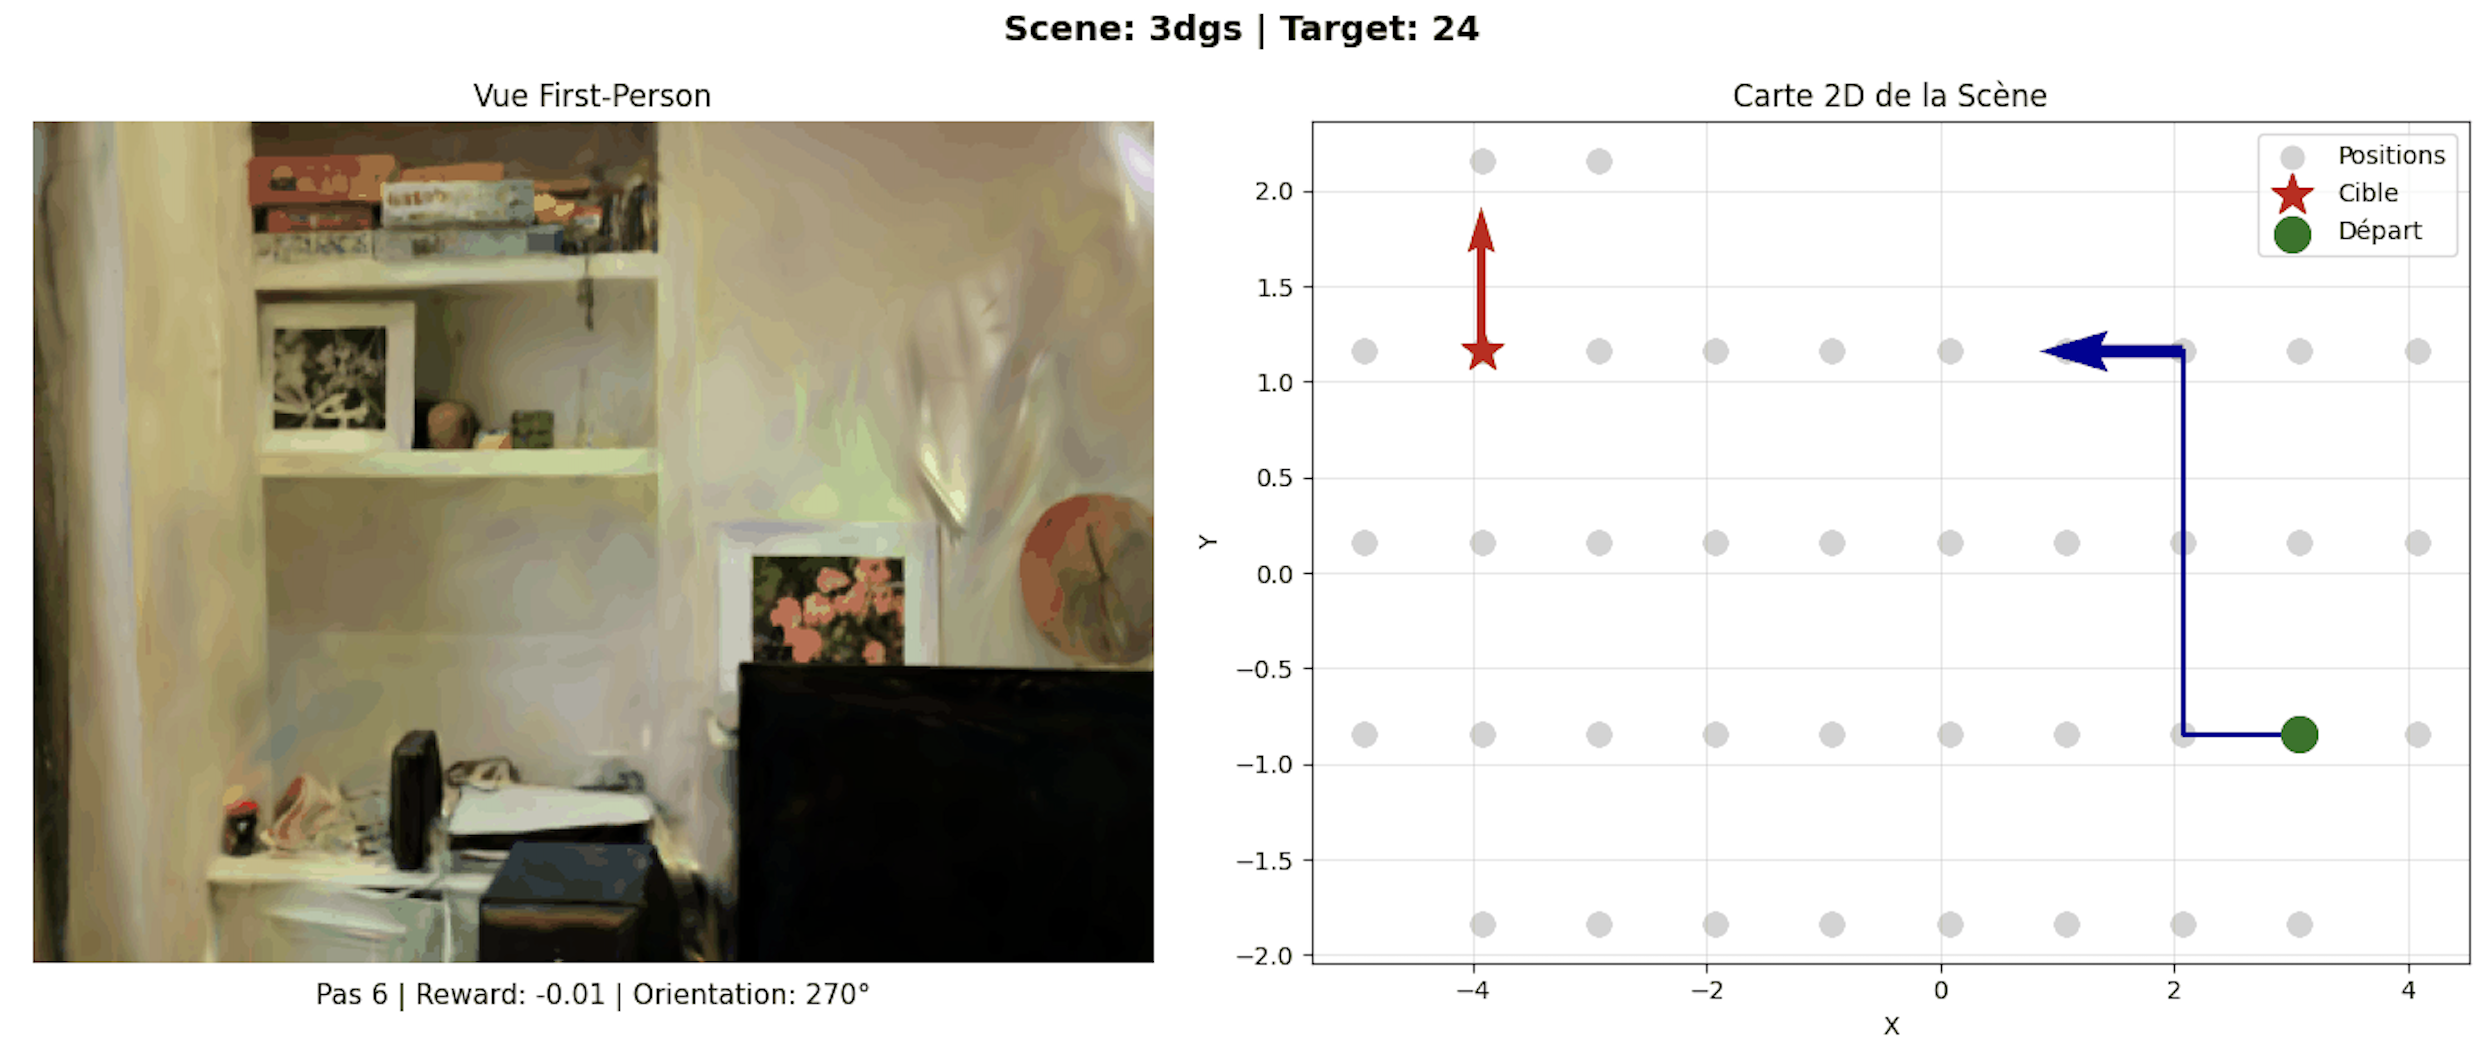
\includegraphics[width=0.8\linewidth]{images/animation_3DGS.png}
    \caption{Exemple de navigation de l'agent A3C sur la scène \texttt{room} (cible 24)}
    \label{fig:animation_3DGS}
\end{figure}

L'agent converge efficacement sur l'ensemble des 5 cibles, avec un 
reward moyen de \textbf{9.92} (proche du maximum théorique de $+10$) 
et une longueur moyenne de trajectoire de \textbf{8.69 pas}. Le taux 
de collisions reste très faible (0.06 en moyenne), ce qui indique que 
l'agent a appris à naviguer de manière fluide dans la scène.

La Figure~\ref{fig:grille_room} illustre la grille de navigation 
construite dans le plan orthogonal à \texttt{up\_world}, avec 
l'enveloppe convexe des poses COLMAP et les nœuds de la grille 
générés à l'intérieur.







\subsection{Approche de navigation continue}
\label{sec:approche_continue}

Cette section est l'extension du pipeline de navigation visuelle  vers un espace d'actions continu. Pour cette phase, nous comparons les algorithmes A3C et PPO sur une tâche de navigation dans la scène \textit{room} reconstruite par le 3DGS. L'environnement est implémenté avec la bibliothèque \textit{Gymnasium}.

\subsubsection{Première phase : comparaison A3C / PPO avec une seule rotation}


Dans cette première version, l'agent reçoit comme entrée un état numérique regroupant sa position courante, la position cible (X,Y,Z), et l'angle de lacet courant(YAW) et cible (normalisés). Il choisit une action continue à quatre composantes.


Les deux algorithmes A3C et PPO ont été entraînés sur cette même tâche, avec le même environnement et la même cible.

\paragraph*{Observations}

Sur cette tâche à une seule rotation, deux constats se sont dégagés de
façon répétée au fil des expériences :

\begin{figure}[H]
    \centering
    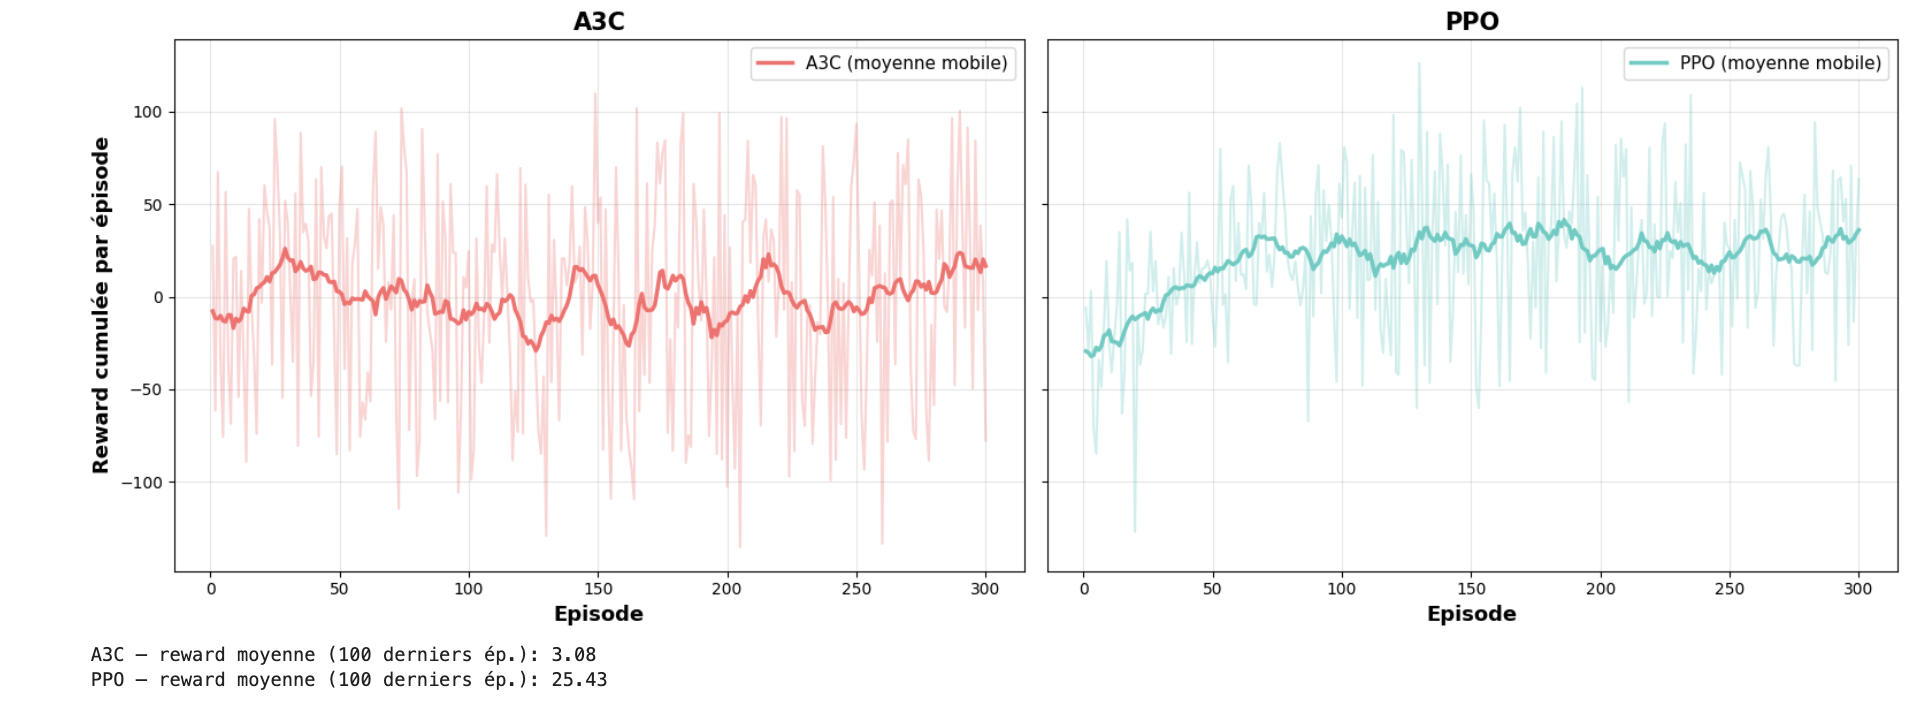
\includegraphics[width=1.0\textwidth]{images/img2.png}
    \caption{Reward par épisode}
    \label{fig:image2}
\end{figure}


\begin{itemize}
    \item \textbf{PPO converge plus vite et de façon nettement plus
    fiable que A3C.} Sur des entraînements de durée comparable, PPO atteint
    systématiquement une distance résiduelle proche du seuil de convergence
    en quelques centaines d'épisodes, avec un temps d'exécution d'une minute pour 300 itérations à 2.1 min pour le A3C.
    \item \textbf{A3C est instable.} 
    
    Sur la même tâche, A3C montre des
    phases de progression suivies d'effondrements soudains de la
    politique --- la distance à la cible remonte brutalement après avoir
    atteint un bon niveau, sans jamais se stabiliser durablement. Ce
    comportement a été observé de façon récurrente, y compris après
    plusieurs ajustements de la récompense et du taux d'apprentissage.
\end{itemize}



\subsubsection{Seconde phase : comparaison A3C / PPO avec orientation complète}



La première version de l'environnement ne représentait l'orientation de la caméra que par le lacet (YAW). Une analyse des poses de caméra réelles du jeu de
données (issues de la reconstruction COLMAP) a montré que le tangage (PITCH) et le roulis (ROLL) varient tous deux de façon importante d'une prise de vue à l'autre,
et ne peuvent donc pas être ignorés si l'on souhaite représenter fidèlement
les orientations réellement présentes dans la scène. L'environnement a par
conséquent été étendu pour que l'agent contrôle les trois rotations de la
caméra, en plus des trois axes de déplacement.

\paragraph*{Architecture}
\subparagraph*{Réseau}
 L'agent est paramétré par un réseau acteur-critique de
type perceptron multicouche (MLP), qui opère directement sur un vecteur d'état numérique plutôt que sur les images rendues par le moteur 3DGS. Ce
choix permet un entraînement nettement plus rapide, puisqu'il évite d'appeler le rendu 3DGS à chaque pas de temps.

Le vecteur d'état, de dimension 12, regroupe :
\begin{itemize}
    \item la position courante de la caméra $\mathbf{p}_t \in \mathbb{R}^3$,
    \item la position cible $\mathbf{p}^\star \in \mathbb{R}^3$,
    \item les trois angles courants (lacet, tangage, roulis), normalisés,
    \item les trois angles cibles, normalisés de la même façon.
\end{itemize}



\subparagraph*{Calcul de la récompense en fonction des trois orientations}

Comme pour la version à une seule rotation, la récompense repose sur un
écart combiné entre l'état courant et l'état cible, qui associe un terme de
position et un terme d'orientation.

\subparagraph*{Terme de position.} Il s'agit de la distance euclidienne entre
la position actuelle et la position cible, normalisée par le diamètre de la
zone de déplacement atteignable par la caméra :
\begin{equation}
    \tilde{d}_{\text{pos}} = \frac{\lVert \mathbf{p}_t - \mathbf{p}^\star \rVert_2}{\operatorname{diam}(\mathcal{P})}
\end{equation}

\subparagraph*{Terme d'orientation.} Deux formulations ont été testées pour ce
terme.

La première combine les trois rotations (lacet, tangage, roulis) en une
seule matrice de rotation par composition, $\mathbf{R} = \mathbf{R}_{\text{yaw}}
\cdot \mathbf{R}_{\text{pitch}} \cdot \mathbf{R}_{\text{roll}}$, et compare
directement les deux orientations complètes via la distance géodésique sur
le groupe des rotations :
\begin{equation}
    d_{\text{orient}} = \arccos\left(\frac{\operatorname{tr}(\mathbf{R}_t^\top \mathbf{R}^\star) - 1}{2}\right)
\end{equation}
Cette formulation, mathématiquement rigoureuse, s'est révélée en pratique
peu exploitable pour l'apprentissage : le couplage non linéaire entre les
trois rotations dans un unique scalaire produit un signal de récompense
dans lequel une amélioration sur un axe de rotation peut être masquée ou
même inversée par une dégradation sur un autre axe, ce qui a systématiquement
empêché la convergence de l'agent sur cette composante, y compris lorsque
l'orientation était isolée de la position dans un environnement de test
dédié.

La seconde formulation, retenue par la suite, calcule un écart angulaire
indépendant pour chacun des trois axes, en tenant compte du caractère
cyclique des angles (un écart entre $359^{\circ}$ et $1^{\circ}$ doit être compté comme
$2^{\circ}$, pas $358^{\circ}$) :
\begin{equation}
    \Delta(\alpha, \beta) = \left| \left( (\alpha - \beta + 180^{\circ}) \bmod 360^{\circ} \right) - 180^{\circ} \right|
\end{equation}
\begin{equation}
    \tilde{d}_{\text{orient}} = \frac{1}{3}\left(
    \frac{\Delta(\psi_t, \psi^\star)}{180^{\circ}} +
    \frac{\Delta(\theta_t, \theta^\star)}{180^{\circ}} +
    \frac{\Delta(\phi_t, \phi^\star)}{180^{\circ}}
    \right)
\end{equation}
où $\psi$, $\theta$, $\phi$ désignent respectivement le lacet, le tangage et
le roulis. Cette formulation découplée, bien que moins rigoureuse
géométriquement, fournit un signal d'apprentissage plus directement
exploitable et a permis d'observer une progression réelle (bien que lente
et sensible aux réglages) de l'agent sur la tâche d'orientation.

\subparagraph*{Écart total et récompense.} Les deux termes normalisés sont
additionnés à parts égales :
\begin{equation}
    D_t = \tilde{d}_{\text{pos}} + \tilde{d}_{\text{orient}}
\end{equation}
et la récompense à chaque pas de temps est proportionnelle à la réduction
de cet écart :
\begin{equation}
    r_t = k \cdot \left(D_{t-1} - D_t\right) + r_{\text{term}} \cdot \mathbb{1}\left[D_t < \varepsilon\right]
\end{equation}


Avec cette formulation, on trouve: 

\begin{figure}[H]
    \centering
    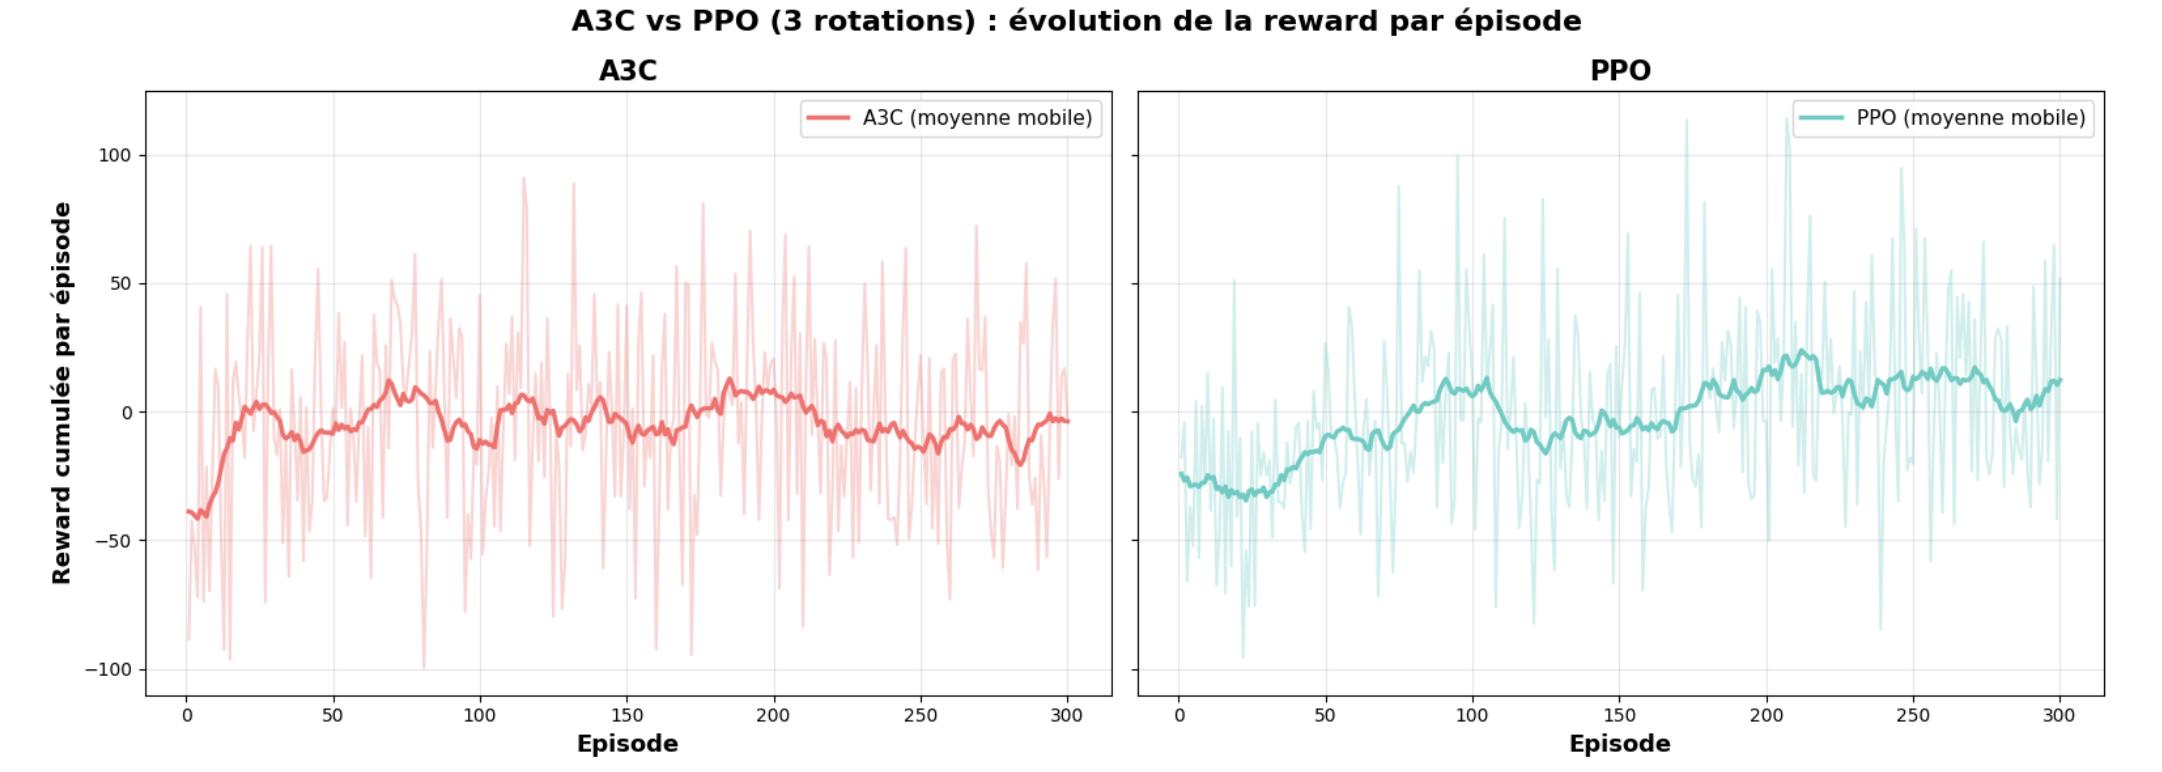
\includegraphics[width=1.0\textwidth]{images/img3.png}
    \caption{Reward par épisode}
    \label{fig:img3}
\end{figure}




Avec l'ajout des trois orientations, on remarque que les deux algorithmes sont
devenus beaucoup moins stables qu'avec une seule orientation, ce qui montre qu'il y a un problème dans la façon d'intégrer ces trois rotations dans le signal d'apprentissage.


\paragraph*{Diagnostic : isolement de l'orientation}

Pour déterminer si l'instabilité observée vient de la coexistence
translation/rotation ou de l'orientation elle-même, un environnement isolé
a été testé : on fixe la position au départ à celle de la cible, seule l'orientation (lacet, tangage, roulis) doit être corrigée par l'agent.

Avec la distance géodésique (équation~30), l'erreur n'affiche aucune tendance de convergence (figure~\ref{fig:orient_geodesic}), confirmant que
la difficulté vient de l'apprentissage de l'orientation, et non de la translation.

\begin{figure}[H]
    \centering
    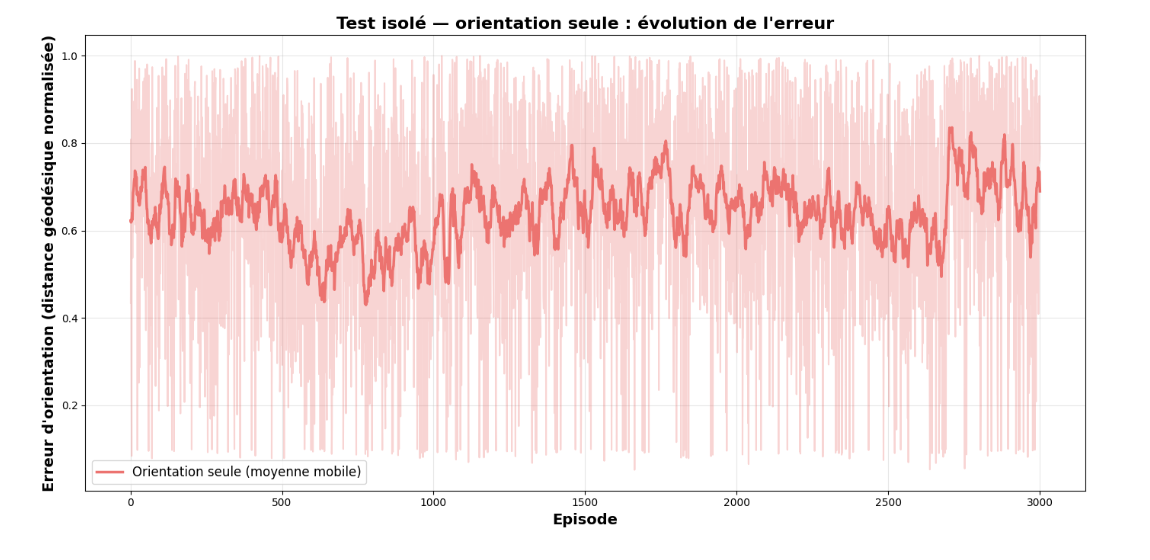
\includegraphics[width=0.7\textwidth]{images/img4.png}
    \caption{Test isolé — orientation seule, distance géodésique}
    \label{fig:orient_geodesic}
\end{figure}

\subparagraph*{Formulation découplée.} Le couplage non linéaire des trois rotations dans un unique scalaire géodésique pouvant masquer un progrès sur un axe par une dégradation sur un autre, une distance découplée a été testée, calculant un écart angulaire indépendant par axe :
\begin{equation}
    \tilde{d}_{\text{orient}}^{\text{découplé}} = \frac{1}{3}\left(
    \frac{\Delta(\psi_t, \psi^\star)}{180^{\circ}} +
    \frac{\Delta(\theta_t, \theta^\star)}{180^{\circ}} +
    \frac{\Delta(\phi_t, \phi^\star)}{180^{\circ}}
    \right)
\end{equation}
où $\Delta(\alpha, \beta) = \left| \left( (\alpha - \beta + 180^{\circ}) \bmod
360^{\circ} \right) - 180^{\circ} \right|$.



\begin{figure}[H]
    \centering
    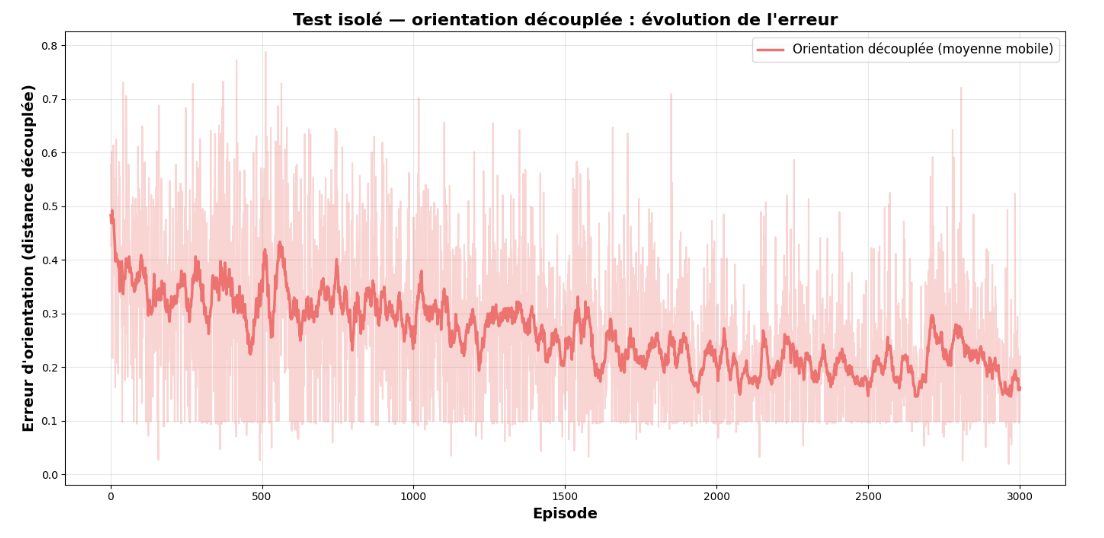
\includegraphics[width=0.8\textwidth]{images/img5.png}
    \caption{Test isolé — orientation seule, distance découplée}
    \label{fig:orient_decoupled}
\end{figure}

Cette formulation permet une progression nette,
de $0{,}45$ à un minimum de $0{,}24$ vers l'épisode 800
(figure~\ref{fig:orient_decoupled}), contre une oscillation sans tendance
autour de $0{,}65$--$0{,}70$ avec la distance géodésique
(figure~\ref{fig:orient_geodesic}) --- confirmant que son couplage non
linéaire freinait bien l'apprentissage. La convergence reste néanmoins
partielle : l'erreur se stabilise autour de $0{,}30$--$0{,}35$ (moyenne
des 100 derniers épisodes : $0{,}3146$), montrant que l'orientation à
trois degrés de liberté reste nettement plus difficile à apprendre que la translation.



\paragraph{Nouvelle représentation de l'orientation : quaternions}

Face à la convergence partielle obtenue avec les angles d'Euler, une
seconde piste a été explorée: 
Cette méthode consiste à représenter l'orientation par un
\emph{quaternion} plutôt que par la composition de trois angles, et
exprimer l'état comme une erreur relative (position et rotation exprimées
dans le repère de la caméra courante) plutôt que comme des poses absolues.
Ce changement de représentation a été testé sur l'environnement complet
(vraies positions et orientations de la scène, cible variable), avec la
même architecture acteur-critique et la même procédure d'optimisation PPO et A3C que précédemment.

\begin{figure}[H]
    \centering
    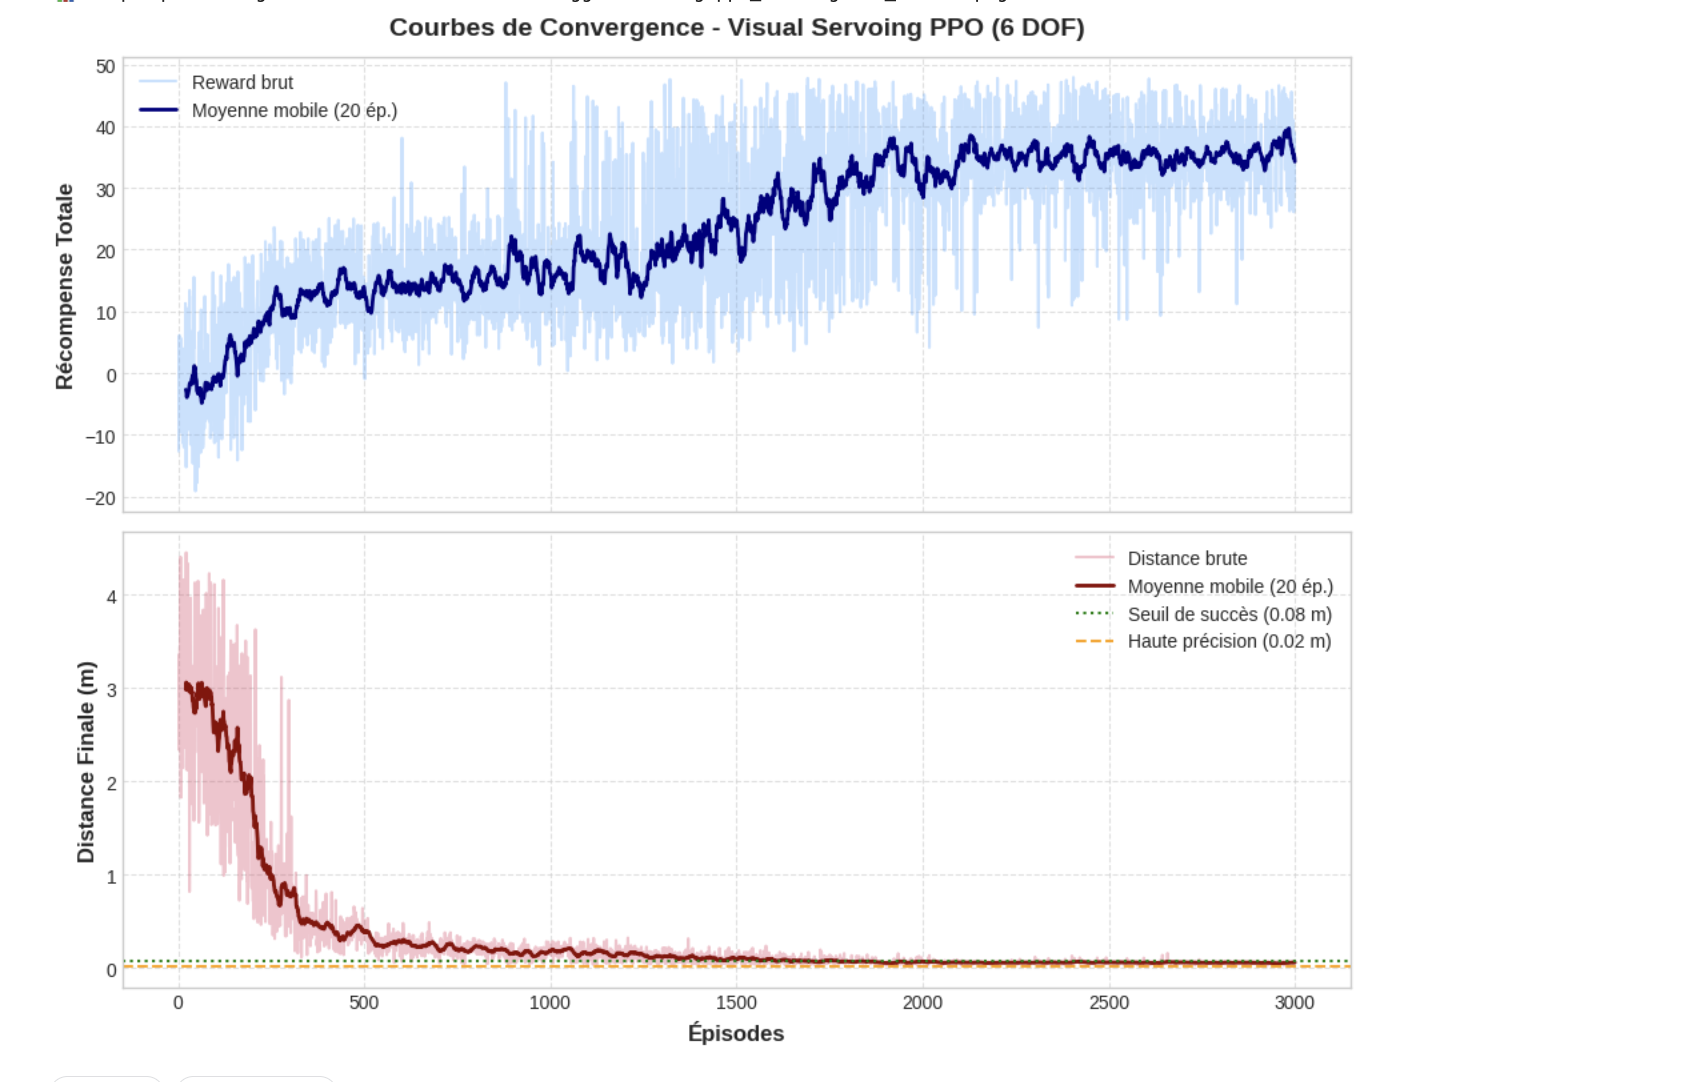
\includegraphics[width=0.8\textwidth]{images/img6.png}
    \caption{Reward et erreur poar épisode}
    \label{fig:img6}
\end{figure}

\begin{figure}[H]
    \centering
    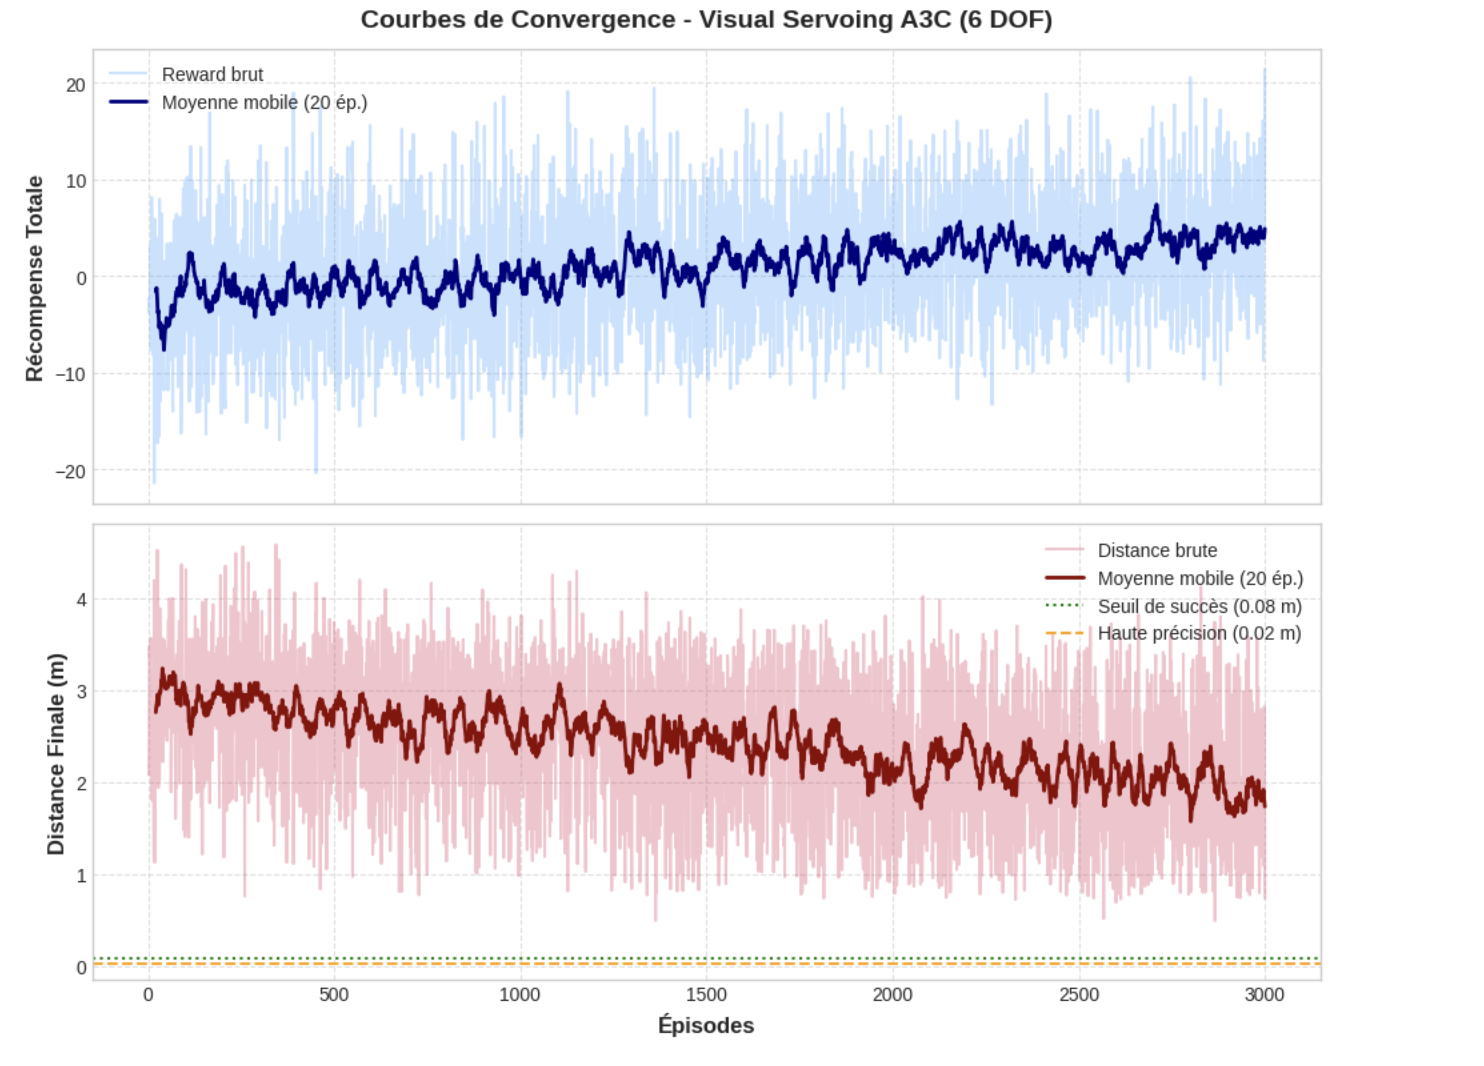
\includegraphics[width=0.8\textwidth]{images/img7.png}
    \caption{Reward et erreur par épisode}
    \label{fig:img7}
\end{figure}



\paragraph{Observations} 

Un premier entraînement avec le PPO sur 3 000 épisodes avec cette représentation a montré une nette amélioration par rapport aux formulations en angles d'Euler : 
\begin{itemize}
    \item la reward moyenne progresse de façon quasi monotone de $0$ à environ $35$--$38$ sur les 3000 épisodes, sans effondrement en fin d'entraînement, contrairement aux essais précédents en angles d'Euler;

    \item La distance finale chute rapidement de $3$ à moins de $0{,}5$ sur les 700 premiers épisodes, puis descend progressivement sous le seuil de succès de $0{,}08$~m à partir de l'épisode $\sim\!1300$, pour finalement se stabiliser en dessous du seuil de haute précision de $0{,}02$~m au-delà de l'épisode $2000$, avec une variance résiduelle très faible. 
\end{itemize}


Contrairement au PPO, l'entraînement avec le A3C montre une progression très limitée :

\begin{itemize}[noitemsep, topsep=4pt]
    \item la reward moyenne (moyenne mobile sur 20 épisodes) progresse 
    légèrement de $-5$ à environ $+4$ sur les 3000 épisodes, mais avec 
    une variance très élevée et sans stabilisation claire ;
    \item la distance finale diminue lentement de $3.1$ m à environ 
    $1.9$ m en fin d'entraînement, sans jamais approcher les seuils 
    de succès ($0.08$ m) ni de haute précision ($0.02$ m), confirmant 
    l'absence de convergence réelle de l'agent.
\end{itemize}

\subsubsection{Troisième phase : observation par image (espace des caractéristiques)}


Les approches précédentes reposaient sur un état numérique décrivant
explicitement la pose (position et orientation) de la caméra et de la
cible. Mais cette dernière était juste la première étape de validation, revenant à une observation
purement visuelle, plus proche de la formulation initiale du problème
d'asservissement visuel : au lieu de comparer les poses, on compare les
\emph{caractéristiques visuelles} extraites des images rendues aux poses
courante et cible.

\paragraph{Extraction de caractéristiques}

Les images rendues par le moteur 3DGS sont passées dans un réseau
convolutif ResNet-18 pré-entraîné sur ImageNet, dont les poids sont gelés. La dernière couche de
classification est retirée, ne conservant que le vecteur de
caractéristiques de dimension 512 produit avant celle-ci, normalisé en
norme $L_2$ :
\begin{equation}
    \mathbf{z} = \frac{f_{\text{ResNet}}(I)}{\lVert f_{\text{ResNet}}(I) \rVert_2} \in \mathbb{R}^{512}
\end{equation}

L'état donné à l'agent est la différence $\mathbf{z}^\star - \mathbf{z}_t$
entre le vecteur de caractéristiques de l'image cible et celui de l'image
courante, plutôt que les deux vecteurs séparément.

\paragraph{Distance et récompense}

L'écart entre l'image courante et l'image cible est mesuré par une
distance cosinus entre leurs vecteurs de caractéristiques normalisés,
mise à l'échelle pour fournir un signal d'apprentissage suffisamment
marqué :
\begin{equation}
    d_{\text{feat}} = \left(1 - \mathbf{z}_t \cdot \mathbf{z}^\star\right) \times 100
\end{equation}
La récompense suit le même principe de différence de potentiel que dans
les formulations précédentes, avec un bonus terminal en cas de succès et
un bonus partiel si l'agent se rapproche suffisamment sans l'atteindre
avant la fin de l'épisode :
\begin{equation}
    r_t = k \cdot \left(d_{\text{feat},t-1} - d_{\text{feat},t}\right) +
    r_{\text{term}} \cdot \mathbb{1}[d_{\text{feat},t} < \varepsilon]
\end{equation}

\paragraph{Architecture et entraînement}

Le réseau acteur-critique reprend la même structure que dans les
approches précédentes, adaptée à une entrée de dimension 512 (le vecteur
de différence de caractéristiques) plutôt qu'un état pose de faible
dimension. L'entraînement suit le même schéma PPO par lots de 10 épisodes
que pour la version par quaternion, avec un plancher de taux
d'apprentissage géré par \texttt{ReduceLROnPlateau}.

\begin{figure}[H]
    \centering
    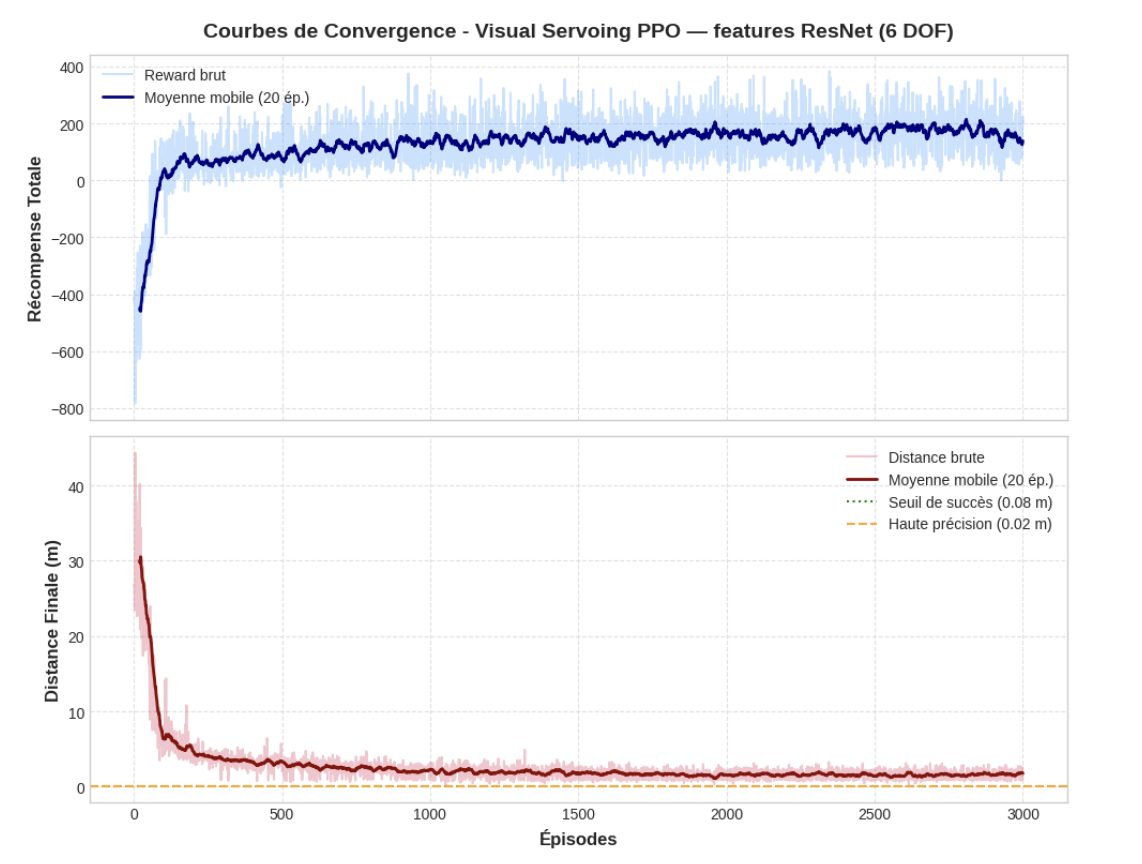
\includegraphics[width=0.8\textwidth]{images/img8.png}
    \caption{Reward poar épisode}
    \label{fig:img8}
\end{figure}

\begin{figure}[H]
    \centering
    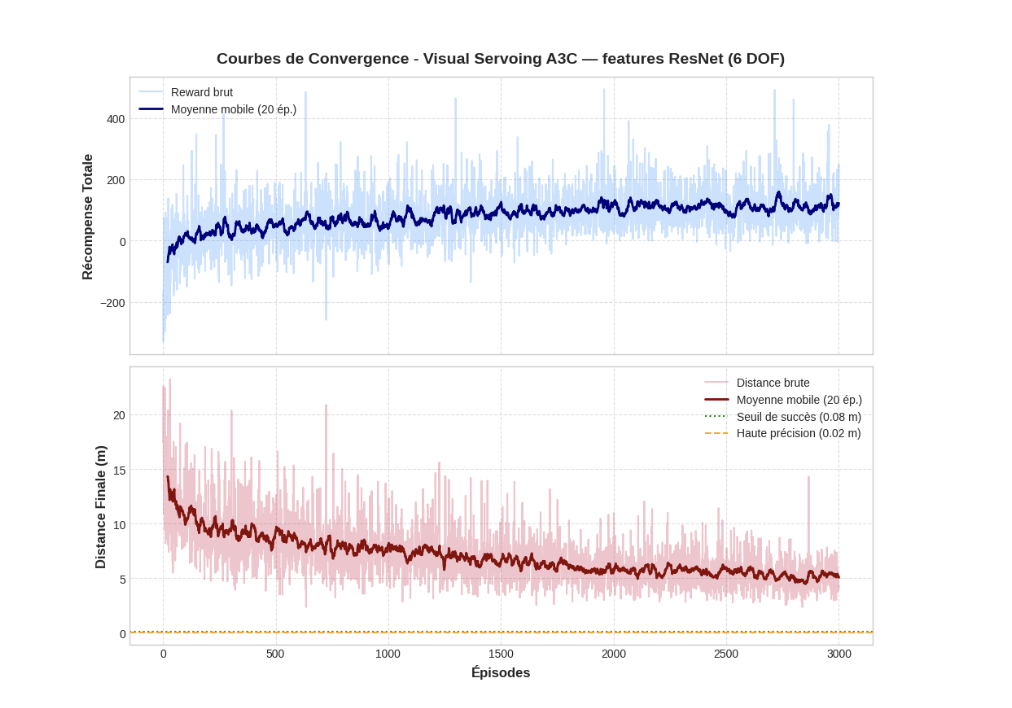
\includegraphics[width=0.8\textwidth]{images/img9.png}
    \caption{Reward poar épisode}
    \label{fig:img9}
\end{figure}

\paragraph{Observations}

\begin{itemize}
    \item La reward moyenne progresse rapidement d'une
    valeur fortement négative en début d'entraînement à un plateau stable
    autour de $80$--$110$, atteint dès l'épisode $\sim\!500$ et maintenu
    jusqu'à la fin des 3000 épisodes, sans dégradation ni progression
    supplémentaire (reward moyenne sur les 100 derniers épisodes :
    $102{,}42$).
    \item Contrairement à PPO, A3C montre une progression très limitée sur cette 
    tâche : la reward moyenne augmente lentement de valeurs très négatives 
    ($\sim\!-200$) à un plateau autour de $130$--$150$, mais avec une 
    variance très élevée tout au long de l'entraînement. La distance finale 
    diminue de $\sim\!13$ m à environ $5$--$6$ m après 3000 épisodes, sans 
    jamais approcher les seuils de succès ($0.08$ m) ni de haute précision 
    ($0.02$ m). Ces résultats confirment, sur la tâche d'asservissement 
    visuel en espace des caractéristiques, la supériorité de PPO sur A3C 
    déjà observée dans les phases précédentes.

\end{itemize}
 

